\chapter{Spielkonzepte/-aspekte mit Einfluss auf die User Experience }
\label{Kapitel:Spielkonzepte}
In diesem Kapitel wird beschrieben, wie in Videospielen Emotionen bei Menschen hervorgerufen werden können. Dazu werden verschiedene Emotionsauslöser beschrieben. Im Anschluss daran wird ein Einblick in verschiedene Spielmechaniken gegeben und die Verbindung zu den Emotionsauslösern dargestellt. %Sowohl der Schwierigkeitsgrad als auch die Rahmenhandlung haben einen weiteren Einfluss auf die Emotionen und somit auf die User Experience. 




\section{Auslöser von Emotionen}
\label{Abschnitt:AuslöserEmotionen}


In jedem Videospielen gibt es viele unterschiedliche Situationen die Emotionen auslösen. Dazu gehören Gefahrensituationen, Veränderungen in zwischenmenschlichen Beziehungen, Erlebnisse die neue Erfahrungen oder Wissen mit sich bringen, besondere Verdienste, die Erlangung eines Wertgegenstandes, Sexualität, zwischenmenschliche Beziehungen, die Beschaffenheit von Landschaften und noch viele weitere. Auch weniger greifbare Elemente wie Musik, Philosophie und Humor gehören dazu. Einige dieser Auslöser sind fest in den Menschen verankert, andere müssen erst gelernt werden. \\
%We have countless different emotional triggers. Physical danger, changes in relationship or social status, learning, strengthening, acquisi- tion of possessions, signs of sexual opportunity, family and safety, and cer- tain types of natural environments are the most obvious, but they’re not the only ones. Humans also respond to music, philosophical ideas, humor and wit, and countless forms of art. Some of these triggers are fixed in our genes. Others can be learned. Most involve complex interactions between conditioning and human nature.
Doch ein Grundprinzip steht hinter jeder Emotion. Eine Emotion kann nur durch eine bedeutsame Situationsänderung entstehen. Eine Emotion bei einer bestimmten Person kann also nur hervorgerufen werden, wenn sich in ihrem Umfeld etwas verändert, dass sie berührt oder beeinflusst.\\
%The bedrock principle behind all emotional triggers is change. To cause emotion, an event must signal a meaningful change in the world. But not just any change will create emotion.
Der \glqq berühmte Reissack\grqq\ , der beispielsweise irgendwo in der Welt umfällt, ruft keine Emotion hervor. Eine Person, die sich im selben Raum, wie der umgefallene Reissack befindet könnte, sich erschrecken oder ärgern, da sie den Reissack wieder aufstellen muss. \\
Ein anderes Beispiel ist in Glücksspielen zu finden. Durch den Gewinn oder Verlust von Geld haben Glücksspiele einen direkten Einfluss auf das Vermögen einer Person. So kann die Spielmechanik bzw. Spielmechaniken solcher Spiele trivial sein und dennoch große Spannung hervorrufen. Eine Person muss also immer persönlich betroffen sein um Emotionen zu empfinden.\\
%In some cases, the changing human value exists only inside the game. Other times, it can be real. For example, gambling games create emo- tion around changes in real wealth. The action of playing craps is fairly boring—players merely roll dice over and over. But when money is riding on the outcome, every roll becomes a nail-biter since it implies a shift be- tween poverty and wealth.
Im Zusammenhang mit Videospielen führt dieser Sachverhalt dazu, dass auch eine Situation der keine große Bedeutung zugemessen wird, der explizite Auslöser für die später empfundenen Emotionen sein kann. \glqq Scouting\grqq\ in einem Strategiespiel wäre ein Beispiel hierfür. Für gewöhnlich bauen in Strategiespielen zwei oder mehr Spieler einen Stützpunkt für eine gewisse Fraktion auf, heben eine Armee aus und bekämpfen sich mit dieser virtuellen Armee, bis nur noch ein Spieler mit seinem Stützpunkt vorhanden ist. Als \glqq Scouting\grqq\ wird das Auskundschaften des Gegners bezeichnet. So lassen sich kommende Spielzüge eines gegnerischen Spielers erahnen. Es werden also weder Einheiten oder Gebäude eines gegnerischen Stützpunktes attackiert noch werden eigene Einheiten produziert oder neue Gebäude gebaut. An sich handelt es sich also um eine Situation in der keine Änderung stattfindet. 
%TeamLiquid
%Scouting is the act of revealing (either with a unit's line-of-sight or Scanner Sweep) remote areas of the map to gain information about the opposing player(s).
%Thus, what is of supreme importance in war is to attack the enemy's strategy.
%~Sun Tzu, The Art of War
%To uncover enemy game-play decisions
%To reveal the expansions of the opponent
%To learn the location of enemy units
%To facilitate the prediction of tech choices
%To assist game-play decisions
%The act of scouting occurs before the game even begins by researching possible enemy builds. Doing this research will increase the effectiveness of scouting and improve your ability to counter the enemy. Researching the possible builds of your enemy will not only show you what he has at the moment of scouting, but what your opponent will have five minutes from then.
Das erkennen von gegnerischen Strategien und die daraus folgende Anpassung der eigenen Strategien entscheidet aber über Sieg oder Niederlage. So kann das erspähen eines bestimmten Gebäudes weitaus emotionaler sein als eine Schlacht bei der zahllose virtuelle Soldaten sterben. Ein Spieler erhofft sich aus dem Erkennen der Gegnerischen Strategie somit den eigenen Sieg. Emotionen können also schon durch die Antizipation (Erwartung) einer Veränderung entstehen. Für jede Situation in der Emotionen erzeugt werden gibt es bestimmte Auslöser:  \cite[S. 11 ff.]{Adams:1515529}
%Even events that seem to be very minor in themselves can be emo- tional if they have important implications. Consider the act of scouting in strategy games. Scouting is no more than seeing an object. It creates nothing, destroys nothing, and moves nothing. By itself it is almost a nonevent. But scouting a strategically important building can reverse a losing game because that one key piece of information can form the core of a new strategy that may lead to victory. So, in a game full of combat and bloodshed, the most emotionally gripping moment might be simply seeing a building.
%
%There are countless ways to create important human value changes in response to even small events. For example, the Modern Warfare series of multiplayer shooters has a kill streak system that hands out special rewards to players who kill a certain number of enemies without dying. 
%
%Emotions don’t just appear in response to a change. They also appear in anticipation of change.
%
%Imagine playing Modern Warfare again. You have counted 10 kills. You know that one more kill will get you the AC-130 bonus and that you’ll likely win the game. In this situation, small local events such as your death or the killing of a single enemy may determine the outcome of the entire match. So you feel suspense because you sense that you are on the knife edge between two drastically different game outcomes. 
%
%S. 11 ff.
\begin{description}

\item[Lernerfolg] - Eine einzige neue Information kann den Unterschied zwischen Verstehen und nicht Verstehen sein. Sie kann auch eine ganze Reihe von neuen Erkenntnissen mit sich bringen. Es verhält sich wie mit einem Puzzleteil, das nachdem es richtig platziert wurde das gesamte Bild erahnen bzw. erkennen lässt. Aber auch die Erkenntnis darüber in die Falle eines Gegenspielers getappt zu sein und die eigenen Fehler zu erkennen ruft positive Emotionen hervor.
\cite[S. 19 ff.]{Adams:1515529}
%leaRning
%Think back to a time when a hard concept finally clicked in your mind. Your eyes light up, your mouth curls into a smile, and the unmistakable expression of epiphany leaves your lips: “Ahhhhhhh!” Learning feels good. 
%
%Insight is the experience of getting a new piece of information that sets off a chain reaction of other lessons. It happens when we get the final piece of a logical puzzle that clicks into place and reveals the shape of the whole.
%For example, in a strategy game, an enemy base is revealed at a spot where you saw some enemy constructors a few minutes earlier. You men- tally kick yourself and say, “I should have known!” Or, in chess, your op- ponent makes a series of seemingly nonsensical moves which later turn out to be a devilish trap that you walked right into. He smiles triumphantly as you say, “I should have known!”
%
%
%S. 19 ff.
% 

\item[Empathie] - Menschen sind mitfühlende Lebewesen. Emotionen, die ein Mensch in einer Situation empfindet, können von anderen Menschen wahrgenommen werden. Darüber hinaus werden sie in der Regel auch unterbewusst gespiegelt. Diese Fähigkeit wird als Empathie bezeichnet. Es bedeutet, dass ein Mensch, der einen anderen vor Freude lachenden Menschen sieht, sich selbst, auch ohne nähere Informationen über die Situation zu haben, glücklich fühlt. Dies gilt auch für Trauer und andere Emotionen. Für Schriftsteller und Drehbuchautoren ist dieses Phänomen ein wichtiges Werkzeug. Es kann somit auch in Spiele mit einem festen Handlungsstrang übertragen werden. In Spielen können solche Situationen aber auch außerhalb der Rahmenhandlung auftreten. Schneidet ein Mitspieler in einer Partie nicht gut ab, können andere Spieler Wut, Mitleid oder Schadenfreude empfinden. \cite[S. 21 f.]{Adams:1515529}\\
Empathie ist zusätzlich der erste Schritt, über die Gefühlswelt einen anderen Menschen kennenzulernen. An dieser Stelle tritt ein Übergang zum ersten Auslöser, dem Lernerfolg auf. Menschen möchten andere, gleichgesinnte Menschen kennenlernen und herausfinden, was ihre Stärken, was ihre Schwächen sind und wie ihre Lebensansichten aussehen. Diese inneren Werte sind besonders deutlich in Ausnahmesituation zu erkennen. Darum werden Protagonisten beispielsweise immer wieder in Situationen dargestellt, in denen sie schwerwiegende Entscheidungen treffen müssen. Für den außenstehenden Betrachter ist dies die Situation in der sich herausstellt, wie gut sie den Protagonisten kennengelernt haben. \cite[S. 21 f.]{Adams:1515529}
%emotion tHRougH CHaRaCteR aRCs 
% Humans are empathetic. See someone smiling, and you’re likely to smile with him. See someone in pain, and you’ll tense up. We mirror emotions we feel in others. This emotional trigger is the stock-in-trade of screenwriters and nov- elists. And like these writers, game designers can predefine character arcs. We can write a story for our game and set it up to play out the same way each time. This is a well-understood and traditional method of provoking emotion, and it can work well.
% 
%But games have another way of creating character arcs: we can have the game generate them on the fly. For example, in a game of Left 4 Dead, three survivors of a zombie apocalypse watch an ally slowly bleed out within sight of the safe room as the monsters lurk nearby. In a game of The Sims, a husband cheats on his wife with a younger woman and gets caught in the act.  
%Character arcs also feed a special kind of learning hunger: we love learning about our peers. We’re particularly interested in the struggles of others, because it is only during conflict that a person’s inner values and abilities are revealed. The more intense the conflict they face, the deeper we see into their true nature. We snore as our hero is forced to choose between skim and whole milk. Force him to choose between his wife’s life and his own, and we stare, wondering who this man will show himself to be.
%
%S. 21 f.
%



\item[Soziale Interaktion] - Allein die Anwesenheit einer weiteren Person ruft in beiden Personen Emotionen hervor. Der Emotionsauslöser Empathie steht damit nicht in Verbindung. Spielmechaniken sind nicht irrelevant, aber je komplexer diese Mechaniken sind desto stärker tritt die soziale Interaktion in den Hintergrund. So reicht beispielsweise ein Ball den sich zwei Spieler gegenseitig zuwerfen als Auslöser dieser Emotionen aus. Diese Emotionen zu benennen ist schwierig. Das Phänomen, dass sich ein Sieg  im Schach  gegen einen Computer anders anfühlt als gegen einen Menschen ist ein Beispiel, das die Auswirkung dieser Emotionen erkennen lässt. Ein Spiel Mensch gegen Maschine ist somit immer emotionsloser als ein Spiel an dem mehrere Menschen teilnehmen. Sobald sich zwei Menschen gegenüberstehen versuchen sie sich gegenseitig zu beeindrucken. Daher ist die Selbstdarstellung eng mit diesem Kriterium verbunden. Durch den Einsatz unterschiedlicher Spielmechaniken lässt sich die Möglichkeit zu Selbstdarstellung verbessern. Schon die Möglichkeit den Spielverlauf in Form von Geistdaten aufzunehmen kann dazu beitragen. Geistdaten sind eine besondere Art von Videoaufnahmen. Hat ein Spieler einen Abschnitt eines Spiels abgeschlossen, wird sein Spielverlauf in das Spiel eines anderen Spielers hineinprojiziert. \cite[S. 22 ff.]{Adams:1515529}

%So kann beispielsweise in Rollenspielen Vertrauen zwischen einer Gruppe von Spielern aufgebaut werden. Dieses Vertrauen ist die Grundlage dafür andere andere Spieler besiegen zu können.
%
%Building trust and breaking it, joking around, defeat- ing strangers, saving friends, and completing a challenge together are all common social experiences that have been designed into games.
%
%Emotionen die durch die anderen Emotionsauslöser hervorgerufen treten stärker in den Vordergrund. 
%
%Wichtig ist nur, dass sich zwei Spieler an einem beliebigen Spiel beteiligen.

%Emotionen lassen sich nicht nur durch eine direkte Verbindung der Gefühlswelten (\textit{Empathie}) auslösen, sondern auch durch zwischenmenschliche Interaktionen. Diese Emotionen können ohne die Hilfe von zusätzlichen Spielmechaniken und nur auf Grund einer sozialen Interaktion ausgelöst werden. 

%or two players create something together, or learn something together, and social interactions are generated around these events
%
%Winning a game of chess against a computer doesn’t feel the same as winning a game against a person, even if the game plays out the same way, because defeating a person adds another layer of emotionally relevant social meaning.
%
%Consider the experience of showing off.Some people’s emotions reward them for showing off, even if the other people involved are strang- ers on the Internet. 
%
%last man alive on your team this round. All of your teammates are observing you, hoping you’ll complete the objective and win the round for them
%
%Any skillful action you take gains another layer of meaning because it reinforces the trust and reputation you’ve built among your teammates. Any mistake you make has the opposite implication. This situation creates knife-edge tension because your social status hangs in the balance.

%emotion tHRougH soCial inteRaCtion
%Catch is a stupid game. At first glance, it’s hard to see why anyone would bother. Players just toss the ball back and forth.  The fact that the game of catch is simple and thoughtless is not a bug; it’s a feature. More complexity would just get in the way of the conversation.
%Catch is the most basic form of socially driven game, since it has almost no emotional content in itself. But most social interaction games use spe- cific game events to drive social interactions. One player defeats another, or two players create something together, or learn something together, and social interactions are generated around these events. Winning a game of chess against a computer doesn’t feel the same as winning a game against a person, even if the game plays out the same way, because defeating a person adds another layer of emotionally relevant social meaning.
%Consider the experience of showing off. Some people’s emotions reward them for showing off, even if the other people involved are strang- ers on the Internet. Imagine a game of Counter-Strike in which you are the last man alive on your team this round. All of your teammates are observing you, hoping you’ll complete the objective and win the round for them. Any skillful action you take gains another layer of meaning because it reinforces the trust and reputation you’ve built among your teammates. Any mistake you make has the opposite implication. This situation creates knife-edge tension because your social status hangs in the balance.
%
%
%Games can support a breathtaking variety of social interactions beyond showing off. Building trust and breaking it, joking around, defeat- ing strangers, saving friends, and completing a challenge together are all common social experiences that have been designed into games. There are a thousand variations on game mechanics that generate social moments. In every case, the social interaction works when it shifts some social human value—stranger to friend, low status to high status, and so on.
%StarCraft and Halo: Reach have replay recording systems that allow players to save, rewatch, and share their greatest victories. Skate has a system for sharing gameplay videos so that a community of players can rate them. Social network games like Farmville allow players to send one
%another gifts or resources that help them achieve objectives. The Sims al- lowed players to share photo-album-like stories about their virtual people. Super Mario Galaxy allows one player to control Mario while another uses the pointing controller to help out by grabbing stars on the screen. Kane & Lynch allows two players to experience its grimy crime story together.
%In a sense, playing a game is a move in the larger game of life. The father who offers to play catch hopes to connect with his son; the internal meaning of catch is less important to him than its use as a tool in life. We play drinking games to establish adulthood. We play chicken with trains to show fearlessness. The middle school boy plays spin the bottle not because he’s interested in probability-based elimination mechanics, but because he knows he might get to kiss the cute girl.
%
%S. 22 ff.
%



\item[Herausforderung] - 
Jede Herausforderung kann ein breites Spektrum an Emotionen verursachen. Der Grund dafür liegt im Schwierigkeitsgrad der Herausforderung. Zu hohe Schwierigkeitsgrade können den Spieler entmutigen, zu niedrige Schwierigkeitsgrade können Langeweile verursachen. Im Idealfall bewegt sich der Schwierigkeitsgrad auf einer Kurve zwischen beiden Extrema. Der Spieler wird im dynamischen Wechsel vor schwierige und weniger schwierige Aufgaben gestellt werden. 
%Dieser Wechsel zwischen Anspannung und Entspannung wird als \glqq Tension-Release\grqq\ bezeichnet. 
Wird diese Kurve eingehalten fühlt sich der Spieler während des Spiels energiegeladen und mächtig. Selbst Fehlschläge rufen in ihm das Gefühl hervor, dass er mit dem  nächsten Versuch aus derselben Situation siegreich hervorgehen wird. \cite[S. 22]{Adams:1515529}\\
Dies macht den Schwierigkeitsgrad zu einem vielseitig einsetzbaren Werkzeug in Spielen. Er ist aber nur einer von vielen Aspekten im Bezug auf die Emotionen. \cite[S. 22]{Adams:1515529}

%Der Schwierigkeitsgrad eines Spiels ist in vielen Fällen der Kern Aspekt im Bezug auf das Erzeugen von Emotionen. Daher so
%Sehr wichtig!
%Schwierigkeitsgrad bzw Kurve wird häufig mit der Qualität des spiels gelcihgesetzt trotzdem gibt es spiele die vollkommen ohne diesen aspekt auskommen und erfolgreich sind wie glücksspiele oder andere spiele auf sozialer interaktion aufgebaut sind.

%emotion tHRougH CHallenge
%Tests of skill and strength create emotions in many ways. As we struggle at them, we enter a pleasurable state of focus. When we pass them, we feel energized, capable, and dominant. Even failure instills a sense of wanting to try again and do better, as long as the player senses the possibility of success.
%Challenge is so closely associated with games that it’s often assumed to be an essential aspect of the medium. It’s part of many common definitions of games. But though it is a powerful and flexible method is still only one more emotional trigger, and not a necessary part of every game design. 


\item[Errungenschaften] - Geschenke und Belohnungen rufen Emotionen hervor. Dies ist der Grund dafür das Menschen sich freuen wenn sie Geld beim aufräumen wiederfinden oder ein Werbegeschenk erhalten. Dies gilt auch für Belohnungen die sie sich erarbeiten müssen. Daher streben Menschen Berufe an die gut bezahlt werden. In Videospielen ist es genau so. Spieler möchten beispielsweise in Rollenspielen immer die beste Ausrüstung besitzen. So können diese Emotionen entstehen wenn sie einen Gegenstand geschenkt bekommen oder sie spezifische Aufgaben erledigen müssen um ihn zu erhalten. Einige Spiele nutzen diesen Auslöser primär und simulieren damit das Gefühl des Reichwerdens. \cite[S. 24]{Adams:1515529} \\ 
Daher ist \glqq ...Diablo III is about the feeling of getting rich.\grqq\ \cite[S. 24]{Adams:1515529} ein Beispiel dafür. %
%emotion tHRougH aCquisition
%We feel a pulse of happiness when we find a dollar under the couch cush- ions. We chase high-paying jobs and freebies. People scream and cry when they win the lottery. Whatever form it takes, acquiring wealth is a bit of a rush.
%Gambling games trigger this response with real wealth. But even games involving no real money can trigger this emotion by creating ar- tificial systems of wealth and acquisition and then giving players wealth within that system. The fake reward still triggers the feeling of acquisition.
%Action role-playing games such as Diablo III are a good example of this. The player wanders around randomly generated dungeons, killing an endless stream of monsters. Defeated demons, zombies, and skeletons spew out little piles of gold, magical weapons, or pieces of armor. Every gold piece and sword contributes to the increasing power of the player’s character. These rewards come so often and so continuously that the player stays on a permanent high of rewards acquisition. The game has narrative, audiovisuals, characters, and challenges, but none of these is its primary emotional driver. At its core, Diablo III is about the feeling of getting rich.
%
%s. 24
%
%
%
%emotion tHRougH musiC
\item[Audio] - Durch den gezielten Einsatz von Musik und Audioeffekten lassen sich beim Zuhörer eine Vielzahl an Emotionen hervorrufen. Darüber hinaus lassen sich Audioelemente ohne großen Aufwand mit verschiedensten Medien kombinieren. Nicht nur Filme und Videospiele nutzen diese Tatsachen, sondern auch Talkshows, Clubs, in Form von Diskotheken und Bars und selbst Diashows werden mit Audiospuren hinterlegt. Die hierbei ausgelösten Emotionen werden nur unterbewusst wahrgenommen. Daher kann eine Person nicht nachvollziehen welches Audioelement beispielsweise aus einem Videospiel, bei ihr welche Emotion hervorgerufen hat. Werden ihr aber einzelne Musikstücke aus genau diesem Spiel vorgespielt, kann sie sich lebhaft an die damit verbunden Spielszenen erinnern. Gerade beim Spielen ist das Gehirn mit der Verarbeitung vieler unterschiedlicher Informationen beschäftigt. So werden viele dieser Informationen nicht im Gedächtnis abgelegt. Die Musik hingegen erzeugt einen kontinuierlichen Fluss an Emotionen und kann somit viel besser in Erinnerung behalten werden. Akzente und Spannungsspitzen in Form von Umgebungsgeräuschen und anderen Audioeffekten können diese Emotionen zusätzlich verstärken, bei zu häufigem Einsatz aber als störend empfunden werden. \cite[S. 24f.]{Adams:1515529}

%Music is a powerful and flexible tool for generating emotion. Since it’s so easy to mix into an experience, it’s used liberally across many media. Films play exciting music during action scenes, nightclubs play sexy music late at night, and daytime talk shows play sad or triumphant songs to empha- size whatever narrative they’re trying to create. Games do the same thing with action, ambient, or scary music.
%
%And music is wonderfully subtle—even more than most emotional triggers. Nobody ever gives it the credit it deserves because nobody con- sciously pays attention to it during play. But even though the conscious mind is oblivious, the unconscious is still processing the music into a continuous flow of feeling. You can tell because music is easily separable from the rest of the experience. Listen to a game soundtrack by itself, and you’ll feel much of what you felt during play. Play the game in silence, and you’ll be surprised at how hollow it feels.
%Nonmusical sounds also create emotion. Screeching metal shoots us full of tension and discomfort. A heartbeat accentuates anticipation. Rain sounds serene. Party whistles are goofy. Squishing fluid suggests disgust. Laying these sounds over other events can accentuate or contrast an emo- tion. But be careful—when overused, such tricks can easily tip into cheesi- ness and end up having the opposite effect.
%
%
%s24f
%
%
%emotion tHRougH sPeCtaCle
\item[Spezial Effekte] - Explosionen und Zeitlupeneffekte sind zwei von vielen Beispielen für spezial Effekte in Videospielen und Filmen. Sie lösen beim Betrachter für einen kurzen Augenblick eine Emotion hervor, die schnell wieder abklingt. Die Kosten für so einen emotionellen Moment sind sowohl in Filmen als auch in Spielen hoch. Dafür entfällt aber die Konstruktion einer Szene mit anderen emotionalen Auslösern, die weitaus aufwändiger zu erstellen sind. Wie die Soundeffekte sollten auch die visuellen Effekte trotz ihrer vielseitigen Verwendbarkeit nicht zu häufig benutzt werden. Sonst verlieren sie zunehmend an Ausdruckskraft und werden belanglos. Im Idealfall findet beispielsweise eine große Explosion nach dem Höhepunkt eines Kampfes statt um diese eine Szene besonders hervorzuheben. \cite[S. 25]{Adams:1515529}
%A Star Destroyer crashes into the Death Star! A super-soldier does a slow- motion dive to dodge an incoming rocket! A tanker truck jackknifes, splits in two, and explodes!
%Razzle-dazzle spectacle can bring a quick emotional rise. Unfortunately, the payoff is shallow and unsustainable. Though these effects are expen- sive to produce, they’re also creatively easy. Other emotional mechanisms like character arcs, socializing, and learning require that we construct interrelated networks of mechanics or characters. Spectacle only requires that something big blow up. As a result, spectacle is often overused by studios long on money and short on creative vigor. In the worst cases, it is used so gratuitously that it crowds out the subtler but more profound sources of emotion.

%Spectacle works when it reinforces what’s already there. When the player has fought through a thicket of fast-moving threats and reached his goal with knuckles white on the controller, it’s probably appropriate that something blow up nice and good. That spectacle works because it accentuates the player’s preexisting sense of relief and accomplishment at winning the battle. The same explosion dispensed again and again outside the context of any challenge leaves players numb.
%
%
%s25
%
%emotion tHRougH Beauty
\item[Schönheit] - Schönheit ist ein weiterer Emotionsauslöser. So können beispielsweise Sonnenuntergänge, lachende Kinder und Gemälde als schön empfunden werden. Die zuvor genannten Beispiele haben keine Gemeinsamkeit. Es gibt also keinen Maßstab um Schönheit zu bestimmen. Eine Person empfindet etwas als schön, wenn sie durch die Wahrnehmung davon emotional berührt wird. Dies ist der Grund dafür, dass bei einigen Schachspielen die Figuren besonders aufwändig geschnitzt oder bei Karten Spielen die einzelnen Karten detailreich illustriert werden. \cite[S. 26]{Adams:1515529} \\
Das Kriterium der Schönheit kann aber auch, genau wie Spezialeffekte, zu häufig eingesetzt und somit belanglos werden. Auf der einen Seite hängt dies mit dem Aufwand der Erstellung von schönen Grafiken zusammen, auf der anderen Seite treten die Spielmechaniken durch die Grafiken in den Hintergrund. Diese verminderte Wahrnehmung kann bis zur Unverständlichkeit des Spiels führen. \cite[S. 26]{Adams:1515529}

%A sunset over the ocean. A healthy, giggling baby. A masterpiece painting. On the surface, these things have nothing in common. But all of them are beautiful. Because beauty isn’t in any particular feature of a thing—it is in how something affects us. Something is beautiful when just perceiving it is pleasurable.
%Games are full of opportunities for beauty. A character can be ren- dered in perfect detail and move with preternatural grace. A world can be painted in just the right color composition. And beauty isn’t limited to video games either—think of the beauty of a well-made chess set, or the painted illustrations on Magic cards.
%But like spectacle, beauty isn’t free, and not just because of the time and artistic skill it requires. The emotions of beauty don’t always fit with the rest of the game. Especially in game about ugly things—depression, horror, or unease—beauty will clash with the rest of the aesthetic. And beautiful art can add audiovisual noise that makes a game harder to un- derstand and interact with.
%As with spectacle, there is a tendency in modern game design to re- flexively inject as much beauty into every situation as possible. But usually, beauty works best when it is channeled toward a specific purpose, not when it is thoughtlessly larded over everything.
%
%s26
%
%

\item[Landschaftstypen] - Unterschiedliche Landschaftstypen rufen starke und verschiedene Emotionen hervor. Diese Emotionen sind angeboren und hängen mit den Fortpflanzungsinstinkten zusammen. Ein Mensch fühlt sich an Orten wohl, die übersichtlich, weder zu kalt noch zu warm sind, die fruchtbaren Boden bieten und somit das Überleben sicher stellen. Abgesehen davon werden auch Landschaftstypen, die dem Landschaftstyp ähneln in der eine Person aufgewachsen ist, von ihr als sicher empfunden. Der Wechsel in die Landschaft einer Spielwelt löst basierend auf diesem Sachverhalt immer Emotionen aus. Diese werden zusätzlich durch Jahreszeiten, Wetter- und Lichtverhältnisse beeinflusst. Die Spielwelten in Videospielen können über diese natürlichen Landschaftstypen hinaus auch surreale Welten erschaffen. So kann beispielsweise durch den Wechsel von einer postapokalyptischen in eine lebensfreundliche Spielwelt das Gefühl von Befreiung und Freiheit beim Spieler entstehen.  \cite[S. 26 f.]{Adams:1515529}
%emotion tHRougH enviRonment
%Lightly wooded grassland feels different from steamy, claustrophobic jungle, which feels different from arctic tundra. And these feelings shift with time and season—winter feels different from summer, night differ- ent from day, rain different from shine.
%There’s evidence that these responses are partly innate. Psychology re- searchers have found that American children shown photographs of vari- ous environments say they would prefer to live in savannas, even though they’ve never been to one. These emotions may reflect an evolutionary imperative to seek out places where a tribe can thrive: fertile, not too hot or cold, not too open or overgrown. The perfect environment for prehistoric humans is open grassland with patches of woods and running water. So when we find a place like this, we feel satisfied and at ease. This emotional reaction draws us into these places where we can reproduce best.
%People also have acquired environmental preferences. We prefer the landscape we grew up in. So, while American children like savannas, American adults also like coniferous and deciduous forests, because those
%
%landscapes resemble much of the United States. And no American in any group wants to live in a desert or rainforest.
%Environmentally driven emotions are diverse and strong. Games have used environments, weather, and season to accentuate feelings ranging from depression to giddy triumph.
%Heavy Rain: This puzzle adventure game is about a man losing his son. In the first few scenes, the world is bright and sunny. But after the boy vanishes, the rest of the game plays out under a downpour, and mostly at night. That endless rain gives every sequence a morose undertone, ac- centuating the themes of loss, crime, and depression.
%Half-Life: Gameplay begins with the player trapped in the giant un- derground Black Mesa facility, so there is no natural light for the first 15 hours of play. When the player finally bursts through the door and onto the sun-drenched New Mexico desert, there’s a palpable sense of freedom and accomplishment.
%Metro 2033: Two decades after the nuclear holocaust, a community of survivors ekes out an existence in the Moscow metro system. It’s dark down there, but people have still made a home. They work, trade, listen to music, drink, and laugh. But the surface is a different story. The vision of Moscow in Metro 2033 may be the least friendly landscape imaginable. Shattered buildings lay frozen in giant chunks of ice. The air itself is toxic, so the player must carry a constantly dwindling supply of gas mask filters. Thousands of icicles menace like spike traps, pulled out sideways by the lashing wind. Everything about the place is endless: the sun never shines, the wind never stops, the ice never melts, and nothing ever grows. I’ll never forget how it felt to pick my way through that rubble. Though most would call Metro 2033 a shooter or a role-playing game, I wouldn’t, because I don’t think it’s about shooting or role-playing. I think it’s about discover- ing how a place like that makes you feel.
%
%s26 f
%
%emotion tHRougH newfangleD teCHnology
\item[Neuheiten] - Erscheint ein neues Videospiel mit neuer bzw. überarbeiteter Grafikengine oder Physikengine ruft es bei Spielern Emotionen hervor. Emotionen die hierbei entstehen unterscheiden sich von Spieler zu Spieler. Denn neue Technologien können sowohl Vorteile als auch Nachteile mit sich bringen. Die Zeit die es benötigt eine Engine zu realisieren fehlt an anderen Stellen die zur Entwicklung eines Spiels benötigt werden, wie zum Beispiel bei den Spielmechaniken. Hinzu kommt, dass den Entwicklern die Routine im Umgang mit der neuen Engine fehlt und diese somit auch nicht in voller Funktionalität genutzt werden kann. Auf Grund dieser Tatsache werden sie häufig abwertend als technologie Demo (\textit{Tech Demo}) bezeichnet. Durchgehend positive Emotionen können daher nur durch neue Technologien entstehen wenn diese direkt an die Spielmechaniken gekoppelt sind. Wird in einem Spiel beispielsweise eine neue auf die Beleuchtung ausgerichtete Grafikengine verwendet, sollte dies mit in die Spielmechaniken einfließen. So können dem Spieler neue Interaktionsmöglichkeiten geboten werden. \cite[S. 27 f.]{Adams:1515529}

%Shiny new tech is cool. The first few games with any new graphics, anima- tion, or physics technology get an emotional rise from certain players just because of the technology itself.
%But this bonus often comes at a cost. Paradoxically, technological ad- vances often lead to a temporary reduction in the design quality of games. This is partially because developers haven’t yet learned how to best use the new technology. More importantly, though, the promise of an easy tech-driven emotional return takes the creative pressure off. So the game
%
%
%becomes a technology demo because it doesn’t need to be anything else to get players excited. The game will still work, for a while. But technological excitement doesn’t last long, and a game that depends on it will not look very good a few years down the road.
%For example, in the mid-1990s it became possible to encode full- motion video on a CD-ROM and play it back on a PC. This technological leap led to some of the worst games in history. These games managed to utterly fail at being movies while simultaneously failing at being games. Although this disaster was driven by many other factors besides tech fetishism (such as the blind theft of creative ideas from film), it was enabled by misplaced trust in technology.
%To achieve sustained success, a game must use its new technology to unlock interactions and situations that couldn’t have been experienced before. For example, Doom is often cited as a technology-driven game because it was the first first-person shooter with varying heights and non- right-angled walls. But Doom did not become a mega-hit just because of its technology. It also took that new technology and used it to unlock a new spectrum of design-driven experiences. Doom wasn’t just the first game with arbitrarily angled walls and changing light levels. It was the first game where demons shut off the lights and charged into the room when you grabbed an item. It was the first immersive horror game where you would hear monsters groaning in the dark and turn in circles, trying to find them. It was the first multiplayer first-person shooter. These elements depended on technology to work, but they are actually advances in game design, and the technology alone did not create them.
%
%s27f
%
%

\item[Urängste] - Die Furcht vor giftigen Tieren, wie Schlangen und Spinnen ist tief in den Menschen verwurzelt. Verseuchte Lebensmittel, Krankheitserreger und lebensbedrohliche Situationen rufen Emotionen in Form von Angst hervor. Die Darstellung dieser Gefahren, selbst virtuell, reicht aus die Emotionen hervorzurufen. Dieser Auslöser lässt sich vergleichsweise einfach benutzen. Auf Grund der Einfachheit wurde er in der Vergangenheit so häufig eingesetzt, dass viele Menschen sich an diese Ängste gewöhnt haben. \cite[S. 28 f.]{Adams:1515529}
In einem der ersten in den Kinos gezeigten Stummfilmen, fuhr eine Dampflock in einen Bahnhof ein. Die Szene war so aufgebaut, dass der Zug auf die Kamera zufuhr. Er wurde auf der Leinwand immer größer. Panik breitete sich untern den Zuschauern aus, sie verließen das Kino. Sie dachten, dass der Zug aus der Leinwand in den Zuschauerraum fährt. \cite[S. 153]{Karasek:1994vb} Durch den häufigen Einsatz dieses Auslösers hat er an Ausdruckskraft verloren. \cite[S. 28 f.]{Adams:1515529}
%emotion tHRougH PRimal tHReats
%Some things have threatened our species for so long that our fear of them is imprinted directly into our genes. Rotten food and disease-ridden filth make us feel revolted to help us avoid food poisoning. Venomous spiders and snakes make us recoil because they’re more dangerous than their size suggests. Visibly diseased people drive us away so that we won’t catch their sickness ourselves. The sight of ghastly wounds kicks off an adrenaline response to prepare us to deal with a dangerous situation. And games can trigger these responses. Just throw gore or spiders on a screen. It’s easy.
%In fact, it’s too easy. The adrenaline rush of these primal threats has been cheapened by decades of overuse by lazy filmmakers and game de- signers. People are just too used to these cheeseball frights by now. Many
%
%
%28f
%

\item[Sexuelle Signale] - Hübsche Gesichter, nackte Haut, verführerische Gesten und Gesichtsausdrücke rufen in Menschen Emotionen hervor. Diese sind, wie die Urängste, tief in den Instinkten des Menschen verankert. Sexualität lässt sich ähnlich einfach wie der Auslöser der Urängste einsetzen. Wird beispielsweise ein Charakter in einem Spiel nackt dargestellt, reicht dies alleine aus, dass Spieler darauf reagieren. Diese Reaktionen können sowohl positiv als negativ sein. Daher sollten sich Spiele, die ein breites Publikum ansprechen wollen, nicht auf sexuelle Inhalte fokussieren. Allgemein gilt, wenn sexuelle Signale zu häufig eingesetzt werden stören sie die Atmosphäre eines Spiels, denn sowohl die Charaktere als auch die Geschichte verlieren an Glaubhaftigkeit. \cite[S. 29f.]{Adams:1515529}
%emotion tHRougH sexual signals
%A game can show some bare skin, a pretty face, an alluring expression, and people will notice because we’re genetically programmed to pay attention to these things. Since these sexual signals are so effective and easy to use, game designers, advertisers, and filmmakers alike have ruthlessly abused them. You can put a mostly naked, attractive character in a game, and some players will respond. As with primal threats, it’s easy.
%But the use of cheap sexual signals has downsides. Gratuitous sexual- ity harms the atmosphere and believability of a serious narrative, and it irritates large classes of potential players (typically the ones not interested in the signals presented). In a certain kind of game made for a certain au- dience, this is fine. For more serious or broadly targeted games, it’s often not worth being tasteless.
%
%29f



\end{description}
%
%






\section{Spielmechaniken}
\label{sec:basis_spielmechaniken}

Spielfiguren und Spielfeld eines Schachspiels lösen bei einem Menschen keine Emotionen aus. Es werden zusätzlich spezifische Regeln benötigt, um bei einem Menschen Emotionen auszulösen. Durch das Regelwerk, indem genau festlegt ist, wie die einzelnen Figuren bewegt werden dürfen, lassen sich Situationen erzeugen, die bei einem Spieler Emotionen verursachen. Die Einhaltung dieser Regeln führt dazu, dass ein Spieler vor Aufgaben gestellt wird, die er lösen möchte. Genau in diesen Situationen, beim Lösen der Aufgaben, werden Emotionen hervorgerufen. Eine Situation könnte so aussehen, dass ein Spieler mehrere Interaktionsmöglichkeiten in seiner Runde hat, aber sich nur für eine dieser Möglichkeiten entscheiden kann. Im Wechselspiel mit einem andern Menschen oder einer Maschine werden so immer wieder Emotionen ausgelöst. In Videospielen wird, im Gegensatz zu Gesellschaftsspielen, zusätzlich zwischen Regeln und Spielmechaniken unterschieden. Eine Spielmechanik ist ein spezieller Typ einer Spielregel. \cite[S. 4 ff.]{Adams:1515529} \\%Sie legt fest, wie ein Spiel bedient wird.
Bezogen auf Videospiele ist die Spielmechanik ein System, mit dem ein Spieler interagiert um Aktionen in einem Spiel auszulösen. \cite[S. 783]{Mattfeld:2012up} \\
Zusätzlich wird durch die Spielmechanik sichergestellt, dass die Regeln des Spiels eingehalten werden. Ein Sprung im Spiel ist z.B. eine Mechanik. Die Geschwindigkeit, mit der sich ein Charakter über den Bildschirm bewegt, hingegen ist eine Regel. Es ist wichtig bereits während der Programmierung des Spiels darauf zu achten, Mechaniken und Regeln voneinander zu trennen. So kann beispielsweise die Mechanik des Sprunges ohne Änderungen in der Programmierung an verschiedenen Stellen in einem Spiel immer wieder verwendet werden. Durch eine Änderung an der Regel, hier der Geschwindigkeit, lässt sich die Höhe bzw. die Weite eines Sprungs beeinflussen. So kann die gleiche Mechanik z.B. in verschiedenen Welten verwendet werden. Diese Welten könnten andere Anziehungskräfte haben, wie beispielsweise der Mond und die Erde. Für den Entwickler ist die Regel also eine Stellschraube für die Spielmechanik\\
In Gesellschaftsspielen sind alle Regeln und Anweisungen, die ein Spieler zum Spielen benötigt, in einer Spielanleitung festgehalten. Auf diese Anleitung kann ein Spieler jederzeit zurückgreifen. Es ist auch möglich, in Absprache mit den anderen Mitspielern, diese Regeln abzuändern. In einem Videospiel hingegen, haben die Spieler weder eine Möglichkeit zur expliziten Einsicht in die Mechanik noch in die Regeln. Es ist dem Spieler somit auch nicht möglich diese zu ändern. Die Aufgabe einer Spielmechanik ist es Ereignisse auszulösen. Ein Ereignis ist eine Situation im Spiel durch die ein Spieler eine Emotion erlebt. \cite[S. 7]{Adams:1515529}
In Abschnitt \ref{Abschnitt:AuslöserEmotionen} wurden die Auslöser für diese Emotionen vorgestellt. Eine Spielmechanik sollte vor der Entwicklung auf mindestens einen dieser Auslöser abzielen. Um beispielsweise die Aufmerksamkeit eines Spielers auf ein bestimmtes Spielobjekt zu lenken, kann der \textit{Spezial Effekt}-Auslöser(\ref{Abschnitt:AuslöserEmotionen}) eingesetzt werden. Ein Beispiel hierfür ist eine Explosion. Die Spielmechanik erzeugt das \textit{Ereignis} der Explosion, der Spieler nimmt diese wahr, wodurch in ihm Emotionen ausgelöst werden. Daraus entsteht in seinem Gedächtnis ein \textit{Erlebnis}. \cite[S. 7]{Adams:1515529} \\
In der Abbildung \ref{pic:mechEreigEmoErlebnis} wird die Entwicklung von einer Spielmechanik bis zum Erlebnis bildlich dargestellt.


\begin{figure}[H]
    \centering
    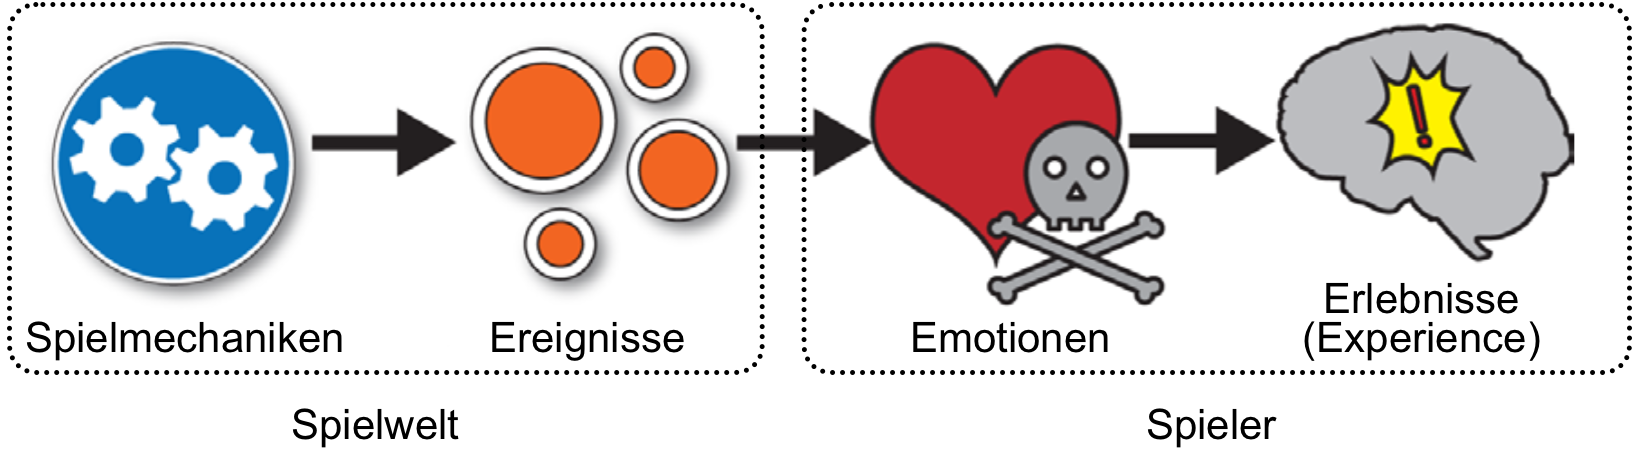
\includegraphics[width=.9\textwidth]{files/games/uxInGames}
    \caption{Einfluss von Spielmechaniken auf die User Experience vgl. \cite[S. 44]{Adams:1515529}}
    \label{pic:mechEreigEmoErlebnis}
\end{figure}


%Viele einfache Spielmechaniken so miteinander zu verbinden, das ein Erlebnis entsteht, wird als \textbf{Emergenz} bezeichnet. \cite[S. 50]{Adams:1515529} 
%Im Kontext von Spiele ist die Spielmeachnik die Kusnst ein Spiel bzw. eine anderes System Spielähnlich zu erschaffen. Spielmechaniken werden damit als Mittel und Anreiz definiert um Aktionen und verhalten von Spielern hervorzurufen und auf die Zeile des Spiels auszurichten. Sie ist damit ein notewendiges instrument damit die Regeln des Spiels umgesetzt werden.

%EMERGENCE is when simple mechanics interact to create complex situations.

%By themselves, chess pieces are just tiny decorative sculptures. But when we move those pieces around according to a special set of rules, those little statues come alive. They will create a nail-biting finish at a high-stakes tournament. They will generate a world of puzzles in the newspaper. They will spark friendships, tell stories, and teach lessons found nowhere else in the universe.

%Reshape the board, add special abilities, change the art, add a story, or make the game play in real time

%A mechanic is a rule about how a game works. The A button makes Mario jump is a mechanic. So are the rules characters walk at one meter per second, pawns capture diagonally, and players alternate taking turns.

%In board games, mechanics are written in the rulebook. In video games, they’re implemented in computer code. But whether the mechan- ics are executed ritualistically by a player or electronically by a computer, they’re still mechanics because they define the game’s behavior.
%During play, mechanics and players interact to generate EVENTS.
%
%\cite[S. 7]{Adams:1515529}

%\glqq To be meaningful, an event must provoke emotion.\grqq\
%

Wird durch das selbe oder ähnliche Ereignisse immer wieder die selbe Emotion hervorgerufen, wirkt dies ermüdend auf den Spieler. Daher muss sichergestellt sein, dass unter der Verwendung verschiedener Spielmechaniken unterschiedliche Ereignisse entstehen. Von Schriftstellern und anderen Autoren wurden daher verschiedene  Spannungskurven entwickelt. In Abbildung \ref{spannungskurve} wird eine häufig verwendete Spannungskurve für Romane und Filme dargestellt. Diese Kurve besitzt zwei Höhepunkte. Der erste Höhepunkt befindet kurz nach Beginn der Handlung, der zweite und noch wichtigere Haupthöhepunkt leitet das Ende der Handlung ein. Diese Kurve kann leicht in die Rahmenhandlung eines Spiels übernommen werden. 
\begin{figure}[H]
    \centering
    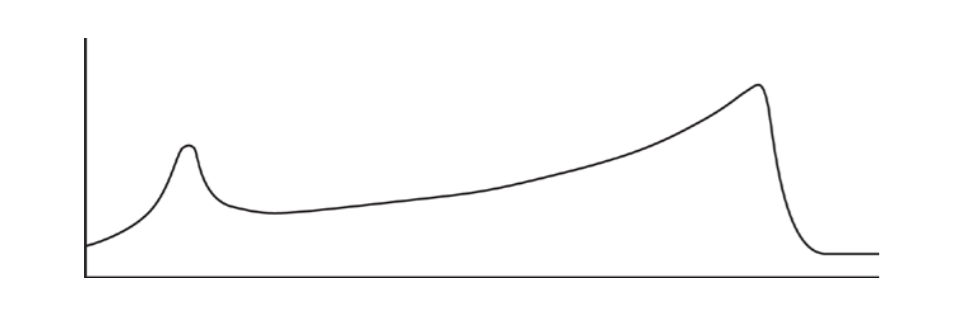
\includegraphics[width=.8\textwidth]{files/games/spannungskurve}
    \caption{Darstellung einer häufig verwendeten Spannungskurve \cite[S. 37]{Adams:1515529}}
    \label{spannungskurve}
\end{figure}

%Sie sollte aber auch von der Spielmechanik automatisch erzeugt werden. 
%Aber die einzelnen Spielmechaniken sollten 
Nicht nur in der Rahmenhandlung, sondern auch durch die Spielmechaniken entsteht eine Spannungskurve. Diese Spannungskurve wird automatisch durch den Spielverlauf mit Spielmechaniken erzeugt. Bei einem Schachspiel kann diese Kurve ähnlich wie in Abbildung \ref{spannungskurve} aussehen. % Die Spannungskurve während eines Schachspiels beispielsweise kann ähnlich aussehen. 
Der erste Höhepunkt, wäre das Schlagen der ersten Einheit im Eröffnungsspiel, und der zweite Höhepunkt, der spielentscheidende Zug, nachdem das Spiel fast beendet ist. Durch die Mechaniken des Sachspiels kann diese Kurve aber auch anders aussehen. Jeder Zug für sich kann ein weiterer neuer Höhepunkt für den jeweiligen Spieler sein. Ein unerwarteter Zug vom Gegenspieler führt zu einer neuen Aufgabe für den anderen Spieler. Ein bereits erwarteter Zug bringt Entspannung. \cite[S. 9]{Adams:1515529}\\
Dieses Wechselspiel von Anspannung, z.B. durch eine neue Aufgabe, die bewältigt werden muss, und Entspannung wird als \textbf{Tension-Release} bezeichnet. \cite[S. 4]{Adams:1515529}\\ 
Das Tension-Release Prinzip findet sich in vielen Spielen wieder. Bei Tetris ist es beispielsweise die Aufgabe des Spielers Blöcke auf dem Bildschirm zu sortieren. Diese Blöcke erscheinen im Spielverlauf immer schneller und füllen den Bildschirm. Indem der Spieler die Blöcke richtig sortiert verschwinden sie wieder. Die Anspannung wird hier durch die schneller erscheinenden Blöcke immer weiter gesteigert. Die Entspannung erlebt der Spieler, wenn die Blöcke wieder verschwinden und er auf die neuen Blöcke wartet.


%4Dadurch das kommende Blöcke, bevor sie beweget werden können, schon angezeigt werden, kann der Spieler planen, wie er den nächsten Block platziert. 

%Die direkte Übersetzung von Tension-Release ist Anspannung und Entspannung. Dieses Konzept ist eines der wichtigsten Werkzeuge, um die Aufmerksamkeit des Spielers aufrecht zu erhalten. Im Grunde bedeutet es, dass der Spieler im dynamischen Wechsel vor schwierigere Aufgaben gestellt werden sollte und darauf folgend die anspannende Situation durch eine einfache Aufgabe aufgelöst werden soll. 


%Imagine playing chess against a stranger. It’s your turn, and you’re losing. You don’t see a good move, so you feel stress and mental strain. As you study the board, the tension mounts. Then, you see your opening: if you jump your knight backward, you can cover your king and threaten his at the same time! Silent relief floods in followed by a sense of accomplishment for solving the puzzle. You make the move, and your opponent grimaces as he realizes what you did. Seeing this, you feel a sense of dominance. Your opponent starts thinking. As you’re enjoying your satisfied glow, you notice a weakness in your position. If he throws his bishop across the board, he can guarantee a capture on your knight. But it’s not an obvious move. Will he see it? Your satisfaction transforms into suspense. Time stretches out as you try to hold your poker face. Finally, your opponent moves a pawn. Relief floods over you again, with even greater intensity than before, as you realize that you’ve got this one in the bag.
%From the outside, this game doesn’t look like much. Two people sat at a table, made strained facial expressions, and quietly moved plastic pieces across a board. Even the players didn’t consciously sense everything they were feeling. But they were experiencing the roller-coaster emotions of competitive chess all the same. And they will come back to get that shift- ing cocktail of emotions again and again.


%\section{Tension-Release-Prinzip}
%Die direkte Übersetzung von Tension-Release bzw. Tension and Release ist Anspannung und Entspannung (auch Erlösung). Dieses Konzept ist eines der wichtigsten Werkzeuge, um die Aufmerksamkeit des Spielers aufrecht zu erhalten. Im Grunde bedeutet es, dass der Spieler im dynamischen Wechsel vor schwierigere Aufgaben gestellt werden sollte und darauf folgend die anspannende Situation durch eine einfache Aufgabe aufgelöst werden soll. 
%Schon die ersten Spiele haben dieses Konzept benutzt um Spannung zu erzeugen. Das lässt sich zum Beispiel auch an dem Spiel Schach feststellen. Bei diesem Spiel ist das Ganze jedoch auch noch an die Prämisse geknüpft, dass Spieler 1 einen Gegner auf einem ähnlichen Niveau hat. Dadurch, dass beide Spieler einen ähnlichen Wissensstand haben, stellen sie sich gegenseitig immer wieder vor schwierigere und leichtere Aufgaben. Dieses Schema lässt sich aber auch noch an einer weiteren Stelle finden und zwar bevor ein Spieler eine Figur des anderen Spieler schlägt, dabei ist der gesamte Weg dorthin mit Anspannung verbunden und im  Moment des Schlagens hört die Anspannung auf und wandelt sich in ein positives Gefühl, da ein angestrebtes Ziel erreicht wurde. 

%TR ist ein grundlegender Auslöser von Emotionen und kann diese vielfältig triggern.
%\cite[S. 9]{Adams:1515529}

%Schon die ersten Spiele haben dieses Konzept benutzt um Spannung zu erzeugen. Das lässt sich zum Beispiel auch an dem Spiel Schach feststellen. Bei diesem Spiel ist das Ganze jedoch auch noch an die Prämisse geknüpft, dass Spieler 1 einen Gegner auf einem ähnlichen Niveau hat. Dadurch, dass beide Spieler einen ähnlichen Wissensstand haben, stellen sie sich gegenseitig immer wieder vor schwierigere und leichtere Aufgaben. Dieses Schema lässt sich aber auch noch an einer weiteren Stelle finden und zwar bevor ein Spieler eine Figur des anderen Spieler schlägt, dabei ist der gesamte Weg dorthin mit Anspannung verbunden und im  Moment des Schlagens hört die Anspannung auf und wandelt sich in ein positives Gefühl, da ein angestrebtes Ziel erreicht wurde. 

%Dieses Prinzip findet sich so gut wie in allen erfolgreichen Spielen. Manchmal muss es jedoch genauer betrachtet werden. Nimmt man z.B. Tetris, so ist es bei diesem Spiel so, dass der Spieler aus Blöcken, die vom oberen Rand des Bildschirms herunterfallen richtig zu stapeln. Die Blöcke haben verschiedene Formen und können u.a. aussehen, wie ein L oder ein Z. Jedoch kann man diese ineinander schieben und somit den Bildschirm Reihe für Reihe füllen. Ist eine Reihe von Links bis Rechts aufgefüllt, verschwindet diese wieder. Dafür kriegt der Spieler Punkte und steigt im Laufe der Zeit Level auf. Je besser ein Spieler ist, desto höher wird das Level, somit fallen die Blöcke schneller nach unten. Dies deckt den Teil der Anspannung ab und jedes mal wenn es dem Spieler gelingt eine oder mehrere Reihen abzubauen, wird die Anspannung wieder gelöst, da der Abstand zur oberen Kante des Bildschirms mit jeder entfernten Reihe wieder vergrößert wird.


Tension-Release kann schon durch simple Spielmechaniken umgesetzt werden. Selbst in einem Videospiel, indem ein Spieler beispielsweise nur die Möglichkeit hat auf eine fixe Position zu schießen, lässt sich das Prinzip von Tension-Release wiederfinden. Es ist ausreichend die Ziele, die er abschießen muss, in verschiednen Zeitabständen voneinander einzublenden. Über die Zeitfenster zwischen dem Erscheinen der Ziele lässt sich dies steuern. Ein rhythmisches Einblenden wäre hier der Entspannungszustand und je arrhythmischer die Einblendungen stattfinden, desto stärker muss sich der Spieler anstrengen sein Ziel zu treffen. Durch die Einführung von Bewegungsmustern, mit denen sich die Ziele über den Bildschirm bewegen, anstelle des Ein- und Ausblendens, ändert sich nichts am ursprünglichen Spiel. Der Spieler kann aber besser wahrnehmen, in welchem Moment er schießen muss, da sich durch diese Mechanik genauer abschätzen lässt, wann das Ziel in der richtigen Position ist. \\
Eine Erweiterung des Zielmechanismus ändert das gesamte Spielgeschehen. Die ursprüngliche Funktion des Zielmechanismus in diesem Beispiel war, je nach Nutzereingabe auf einen fixen Punkt zu schießen. Wird es dem Spieler aber erlaubt den Punkt, auf den er zielt zu manipulieren, können völlig neue Situationen entstehen. Es entstehen Ziele, die ein Spieler nicht rechtzeitig erreichen kann, da er zuvor bzw. gleichzeitig ein anderes Ziel verfolgt. Es kann passieren, das ein Spieler ein Ziel nicht erkennt, da er zu sehr auf ein anderes Ziel fixiert ist. Spiele wie \glqq Duckhunt\grqq\ für das Nintendo Entertainment System und \glqq Moorhuhn\grqq\ für den PC basieren auf diesen Mechaniken. Durch die Realisierung weiterer Mechaniken kann die Vielfalt der erzeugten Ereignisse weiter vergrößert werden. \\
Die Bewegungsmuster, die bereits für die Ziele, die ein Spieler treffen muss, verwendet werden können auch für den virtuellen Spieler benutzt werden. So kann die Illusion beim realen Spieler entstehen, das er sich durch eine virtuelle Welt bewegt. Zum einen wird so das Zielen beeinflusst, zum anderen entsteht so die Möglichkeit den im Spiel angezeigten Hintergrund mit zu verändern. Spiele dieser Art werden als \glqq Rail Shooter\grqq\ bezeichnet, da der Spieler wie bei einer Achterbahn- oder Zugfahrt wie auf Gleisen durch das Spiel bewegt wird und keinen Einfluss auf die Geschwindigkeit hat. Den Spielen der \glqq Virtua Cop\grqq\ oder \glqq House of the Dead\grqq\ Reihe von \glqq Sega\grqq\ liegen diese Mechaniken zu Grunde. Dadurch das die Spieler durch die Welt geführt werden lässt sich ähnlich wie bei einem Film die Rahmenhandlung mit dem bewegten Bild verknüpfen. Die Mechaniken der Spielerbewegung kann aber auch so abgeändert werden, dass der Spieler sich selber frei in der Spielwelt bewegen kann. Dadurch bekommt der Spieler selber die Möglichkeit sich auf Gegner zu zu bewegen, um so beispielsweise Treffergenauigkeit zu erhöhen oder von ihnen weg zu bewegen, um den Gegnern besser auszuweichen. Dieses Spielgenre wird als \glqq Ego-Shooter\grqq\ bezeichnet. Spiele dieses Genres sind stark vertreten. Die einzelnen Spiele unterscheiden sich nur im Szenario. Die zu Grunde liegenden Spielmechaniken, schießen, umschauen und bewegen bleiben die selben und werden in den Spielwelten in verschiedenen Zeitaltern und vor unterschiedlichen Rahmenhandlungen präsentiert. \cite[S. 50 f.]{Adams:1515529}


%Werden die Mechaniken die die Bewegungsmuster vorgeben und so einen Spieler durch die Spielwelt führen so abgeändert, dass sich der Spieler selber frei durch die Welt bewegen 
%Eleganter ist es aber, wenn 
%Schussmechanik für sich alleine: Ein knopf drücken, schuss. 2 möglichkeiten treffer verfehlt , timing
%Betrachtngsmechanik zugfahrt oder achterbahn, erkundung der landschaft mit den kamera perspektiven 
%beide zusammen ist keine einfach addition, während man schieß erkennt man von der landschaft nicht mehr so viel gegner befinden sich außerhalb des bildschirms gegner priorisieren : look n shoot:  house of the dead (railshooter)
%Bewegungsmechanik: spieler können sich in einer spielwelt frei bewegen und in alle richtungen schießen. spieler hat die möglichkeit gegnern auszuweichen, sich auf die gegner zubewegen um die wahrscheinlichkeit einen treffer zu erzielen zu erhöhen oder einfach nur die spielwelt erkunden.
%Jedes jahr erschienen zahlreiche die auf dieser Spielmechanik basieren. szenario, wie zeit und hintergrundgeschichte variieren, jedoch sind es vom kern die identische spielmachnik. schießen, umschauen bewegung
%somit können viel verschiedene spiele relativ einfaych entwickelt werden, und die verschiedenen spieldesinger müssen nur ein paar zusätzliche mechaniken implementieren, damit sich die spiel voneinander unterscheiden. Für die spieler hat es den vorteil, das sie das wissen aus anderen spielen übernehmen können und nciht viele neue bedienkonzepte erlernen müssen. und schon ist wieder ein neues system erstellt, das die spieler triumpf, sorge, spannung spaß fühlen lässt. \cite[S. 50 f.]{Adams:1515529}

%A shooting mechanic can exist alone. For example, imagine a game in which you time shots from an unmoving cannon to hit enemy planes as they fly past. This game has only one control: a fire button. And it produces a few types of simple experiences. You shoot and miss, or you shoot and hit.
%A looking mechanic can also exist alone. Imagine a roller-coaster sim- ulator in which your only interaction is looking around. Again, you have one control: a joystick for the camera. And again, there isn’t much breadth of experience. Once you’ve looked in every direction on every roller-coaster ride, there’s nothing left to do.
%Now imagine combining these mechanics in one game. You can ride the roller coaster, look in any direction, and shoot at planes flying S.50
%past. This combination doesn’t just add up the experiences of looking and shooting. It multiplies them into a combinatorial explosion of new emer- gent possibilities. We can create aiming challenges where there were none before. Players have to trade off targeting one enemy over targeting an- other. The player might even have to learn situational awareness to know where to look for targets off-screen. This simple look–shoot combination is so elegant that it drives countless games, from The House of the Dead to Space Invaders.
%Now imagine adding a movement mechanic. The player can run around an environment, looking and shooting in any direction. The number of possibilities multiplies again. Now the player can move around to dodge attacks, rush forward to attack, or explore a space to learn about its story. Games designed around this simple combination of shoot, look, and move earn billions of dollars every year. They vary tremendously in their fiction and emphasis: in one, you’re a space marine blasting aliens; in another you’re exploring a somber underwater city. But all these games share the same elegant core: shoot, look, and move.
%And those millions of different play experiences come at a remarkably low cost. The designers need only implement a few mechanics. The play- ers need only learn a few controls. Once that’s done, a million variations of triumph, sorrow, tension, and joy will emerge. S. 51

%\subsection{Eleganz} 
%\label{Abschnitt:}

Nicht alle Spielmechaniken greifen so in einander, wie die Basis Mechaniken für \glqq Shooter Spiele\grqq\ . Gerade in Rollenspielen in denen es viele unterschiedliche Gegenstände gibt, mit denen ein Spieler interagieren kann, wird das Zusammenspiel der Mechaniken komplex. In der Regel kann ein Spieler in so einem Spiel mit verschiedenen Gegenständen ausrüsten. Dazu gehören nicht nur Waffen wie Schwerter, Speere und Bögen sondern auch Zauber, Rüstungen und vieles mehr. Alle diese Gegenstände gehören neben anderen Kategorien zu einer Kategorie in dessen Zentrum das Thema Schaden steht. Waffen und Zauber können Schaden verursachen, Rüstungen können Schaden verhindern. Im Spiele interagieren so die Angriffs- und Verteidiungswerte miteinander. Damit die Gegenstände nicht als langweilig empfunden werden, besitzen sie unterschiedliche Werte. An dieser Stelle tritt das Problem der Komplexität in den Vordergrund. Verursacht eine Waffe zu viel Schaden bei einem bestimmten Rüstungstyp, gibt es zwei Lösungsansätze. Einer wäre, den Schaden der Waffe zu reduzieren, der andere wäre die Verteidigung der Rüstung zu erhöhen. Da sich diese Gegenstände aber in einem Netz mit vielen anderen Gegenständen beeinflusst diese eine Änderung alle anderen Gegenstände. Macht die eine Waffe weniger Schaden, kann es sein, das sie im Gegensatz zu den anderen Waffen irrelevant für den Spieler wird. Wird die eine Rüstung verstärkt, müssen evtl. andere Waffen und Rüstungen angepasst werden, damit die eine Rüstung nicht viel besser als die anderen Rüstungen ist. Durch verschiedene Zauber beispielsweise werden die Beziehungen zwischen den Gegenständen erneut komplexer. So könnte z.B. ein Feuerball Schaden über eine größere Fläche als ein Schwert verbreiten und zusätzlich bestimmte Gegenstände entzünden. Eine Möglichkeit besteht die Abhängigkeiten zwischen den Gegenständen zu reduzieren. Indem für jeden Gegenstand bei der Entwicklung festgesetzt wird wie er jedem anderen einzelnen Gegenstand interagiert. Dies ist aber ein großes Problem in der Entwicklung, da Programmcode der theoretisch beiseite gelegt werden kann und nicht mehr überarbeitet werden muss, jedes mal angepasst werden muss, wenn ein neuer Gegenstand zu einem späteren Zeitpunkt, ins Spiel eingefügt werden soll. \cite[S. 51 f.]{Adams:1515529}
%Als Eleganz wird das zusammenspiel einzelner Spielmechaniken bezeichnet. Idealerweise ist die dieses zusammenspiel etwas komplexer, so dass der zusammenhang nicht direkt ersichtlich ist. schwer zu erreichen

%zusammenarbeit: laufen umschauen und schießen funktioniert daher so gut, da es ohne große umstände vom spieler gleichzeitig bedient werden kann. 
%diese mechaniken sind zusätzlich so verbunden, dass die abgeändert werden können, langsam laufen, bei verletzung, kamera einschränken...
%probleme enstehen an stellen, an denen zu viele mechaniken voneinander abhängen.

%gegestand zu effektiv gegen gegner A 
%Möglichkeit: 
%gegenstand  Angriff --
%gegner verteidigung --
%andere gegenstände oder andere gegenstände ?? 
%1 gegenstand -> 1 gegner = keine probleme

%Spiele mit einem gegenstandssystem haben ein komplexes netz an beziehungen
%viele weitere möglichkeiten was ist wenn ein gegenstand schaden in der umgebung des spielers verursacht, was passiert mit freundlichen mitspielern

%komplexe netze sind nur sehr schwierig zu handhaben, für einfachheit immer nur einen gegenstand pro gegner, nicht elegant immer neue sachen  s.51f.

%Elegance happens when mechanics interact in complex, nonobvious ways. But this same complexity and nonobviousness makes elegant design very difficult to achieve.
%Elegance requires that different mechanics interact. For example, the look, shoot, move combination works well because the player uses all of these controls at once. Since the mechanics all work together, they can multiply into many different possibilities. But this tight interaction be- tween mechanics also makes it hard to solve design problems because changes in one mechanic also affect all the others.
%In an inelegant game, isolated problems are easy to fix. If the wizard’s goblin-killer rod is too powerful when used against goblins, the designer can just reduce its power. Since the rod has no effect on anything besides goblins, this change has no side effects and the problem is solved.
%But this easy solution is only possible because the design is so in- elegant. Why can’t you use the rod against orcs, ogres, other wizards, the   s.51 gods, or stingy shopkeepers? A wizard’s rod implies a universe of possibili- ties in a fantasy world. Limiting it to goblins loses most of them.
%A more elegant game would allow all of these interactions, creating many more play situations without much more learning burden. But this creates a challenge for the designer. Now that the wizard’s rod is con- nected to so many other parts of the game, changing it changes all those relationships. Powering it down might balance it against goblins but make it too weak against orcs. Giving it an area of effect explosion may create exciting field combat but make the rod too dangerous to use near allies. These kinds of problems can get very thorny as the number of relation- ships increases into the hundreds or thousands.
%This is why simple, elegant games are so uncommon. Crafting a system of relationships is much harder than authoring a series of one-off gimmicks, but it’s the only way to get a lifetime of play experiences from a handful of game mechanics. s.52
%Sensing elegant mechanics is much the same. A designer can’t pre- dict every outcome that an elegant game will create. They are too numer- ous and too fuzzy. We can implement the mechanic and test it heavily, but this can take a lot of time. We need ways to spot elegance on the drawing board. And the only real way to do that is to smell elegance the same way my professor smelled invertible matrices: by using trained intuition and mental heuristics.

Die einzelnen Mechaniken für die Gegenstände arbeiten auf engem Raum miteinander, sie vermischen keine Spielkonzepte miteinander. In anderen Spielen können die Spieler aber beispielsweise mit einem Flugzeug durch die Luft fliegen, während andere sich Spieler nur zu Fuß oder mit Fahrzeugen am Boden oder im Wasser bewegen können. In so einem Spiel müssen eine Vielzahl von Mechaniken und Regeln angepasst werden, damit nicht nur eine Spielweise von den Spielern präferiert wird.\cite[S. 55]{Adams:1515529}

%-Spielkonzepte mixen\\

%Doch ist nicht jede Idee praktikabel und umsetzbar oder wird vielleicht durch andere Ideen obsolet. [Zitat] Bsp.: Gibt man einem Spieler die Möglichkeit sich in bestimmten Mustern über den Bildschirm zu bewegen und dem anderen Spieler die Fähigkeit großflächig schaden anzurichten, (Fußsoldat und Kampfjet) hat dieser einen unfairen Vorteil, der vielleicht auf den ersten Blick gar nicht auffällt. Daher muss man sich bei der Kombination verschiedener Spielelemente stets darüber im klaren sein, was man damit erreichen möchte...

%S. 55

\section{Schwiergkeitsgrad} 
\label{Abschnitt:Skill}

Alle Videospiele haben unterschiedliche Schwierigkeitsgrade. Je besser der Schwierigkeitsgrad eines Spiels an die Fähigkeiten, des Spielers angepasst ist, desto stärkere Emotionen können durch das \glqq Tension-Release\grqq\-Prinzip hervorgerufen werden. In Abschnitt \ref{Abschnitt:AuslöserEmotionen} wurde bereits erläutert, dass durch Herausforderungen ein breites Spektrum an Emotionen erzeugt wird. Um diese Vielfalt an Emotionen hervorzurufen, muss die Spielmechanik die Voraussetzung dafür bieten. Einfache Spiele werden schnell langweilig, zu schwere Spiele lösen Frustration aus. \cite[S. 63]{Adams:1515529}




%Zu einfach langweilig, zu schwer frustierrend, daher dazwischen s.63

%Unter und obergrenze besser verstehen

\begin{description}


\item[Tiefgang] - Je schwieriger es ist ein Spiel zu beherrschen, desto mehr Tiefgang besitzt es.  Zu wenig Tiefgang macht ein Spiel trivial. Beim Spiel \glqq Tic Tac Toe\grqq\, häufig auch \glqq XXO \grqq\ oder \glqq Drei gewinnt\grqq\ genannt, zeichnen zwei Spieler abwechselnd je ein Symbol auf ein 3x3 Rasterspielfeld. Das Symbol des ersten Spielers ist in der Regel ein \glqq X\grqq\ und das des zweiten Spielers ein \glqq O\grqq\ . Sobald ein Spieler drei Felder, horizontal, vertikal oder diagonal mit seinem Symbol gefüllt hat, gewinnt er das Spiel. Bei diesem Spiel gibt Strategien, die dem ersten Spieler den Sieg sichern. Diese Strategien sind leicht zu erlernen. Somit hat das Spiel wenig Tiefgang und wird schnell langweilig. Spiele wie Schach, Poker und Strategievideospiele hingegen haben viel Tiefgang. Die Spieler müssen verschiedene Regeln und Spielzüge erlernen und selbst nach jahrelanger Übung gibt es immer wieder Situationen, in denen die Spieler neue Strategie entwickeln müssen. Das entwickeln von neuen Strategien ist dabei besonders schwierig, da die Basis Regeln in Gänze verstanden sein worden müssen und zusätzlich viel Spielerfahrung nötig ist. Der Tiefgang eines Spiels kann grob bestimmt werden, indem perfekte Züge mit den Zügen eines Spielers verglichen werden. Bei \glqq Tic Tac Toe\grqq\ kann der Spieler schnell die perfekten Züge erlernen. Beim Schach hingegen, können selbst Schachmeister von modernen Schachcomputern geschlagen werden. Es gibt somit potenzielle Strategien, die selbst von Schachmeistern noch erlernt werden können. Strategievideospiele basieren in der Regel auf ähnlichen Grundprinzipien wie Schach. Durch die Übertragung in die virtuelle Spielwelt gibt es zahllose Möglichkeiten diese Grundprinzipen durch weitere Spielmechaniken zu erweitern, so kann noch mehr Tiefgang entstehen. Während Schach rundenbasiert ist, d.h. die Spieler führen abwechselnd einen Zug nach dem anderen aus, laufen viele Strategievideospiele in Echtzeit. Echtzeit bedeutet, dass die Spieler gleichzeitig ihre Aktionen ausführen, es gibt also keine Spielzüge bzw. Runden. Dadurch entsteht eine zusätzliche Dimension des Tiefgangs. Der Spieler muss jede seiner Aktionen im Spiel zeitlich optieren, während er auf die Aktionen des Gegenspielers reagiert. Spieler mit einem schnelleren Reaktionsvermögen sind dadurch in einigen Situationen im Vorteil. In Spielen die als \glqq Ego-Shooter\grqq\ bezeichnet werden ist die Reaktionszeit das wichtigste Spielelement, für den Tiefgang. Strategieentwicklung ist in diesen Spielen auch vorhanden, rückt aber oft in den Hintergrund. Der im Vordergrund stehende Vorgang des Zielens und Schießens kann optimiert werden und bringt den Tiefgang in diese Spiele. Ein Computer kann diesen Vorgang perfekt berechnen, er ist schneller und präziser als ein Mensch. Auch Menschen haben unterschiedliche Reaktionszeiten. Es gibt somit immer Verbesserungspotenzial, also Tiefgang. \cite[S. 63 ff.]{Adams:1515529}   
    
    %Die Ironie dabei ist, Spieler stets mit aller Macht versuchen ein Spiel zu schlagen, 


% Als Tiefgang wird 
%steht in verbindung mit dem tiefgang eines spiels. viel tiefgang: viel zu erlernen. schach, poker strategiespiele = viel tiefgang. bei diesen spielen lernen die spieler über sehr lange zeiträume immer neue möglichkeiten das spiel zu spielen. tic tac toe das gegenteil, es gibt ein oder zwei tricks, mit denen man die meisten spiele gewinnen kann.

%ironie: spieler versuchen mit allen mitteln ein spiel zu schlagen, haben sie dieses geschafft bietet das spiel aber nichts mehr für sie. 
%freuen sich, wenn sie ihr geschick verbessern und etwas schaffen was sie am vortag nicht geschafft haben. ein durchgespieltes spiel ist wertlos. es gibt nichts zu lernen, keine ungewissheiten, keinen verdienten sieg und keine niederlage.

%Um den Tiefgang eins spiels zu bestimmen gibt lässt sich so gestalten. vergleich zwischen perfekten aktionen und den aktionen die ein mensch im bestmöglichen fall durchführen kann. so lange es situationen gibt in denen der spieler fehler macht, gibt es etwas für ihn zu lernen. dies nur schwer verständlich. daher beispiel: schach: mensch gegen computer, selbst großmeister verlieren gegen schachcomputer daher haben sie noch nicht die obergrenze erreicht und können somit immer noch etwas lernen.

%Selbes phänomen in shootern, bewegung zielen schießen. es ist möglich alle gegner in wenigen sekunden zu besigen, aber nur theoretisch möglich
%noch einmal tic tac toe es lässt sich mit ein oder zwei schritten immer schlagen oder zumindest ein unentschieden erreichen. somit wird es danach langweilig. ein spiel das in der mitte dieser beiden extrma liegt muss muss zusätzliche emotionale auslöser bieten und durch eine detaillierte darstellung oder eine umfangreiche hintergrundgeschichte angereichert sein.

 %any game that uses challenge—and most do—must deal with the issue of player skill. A challenge that is too hard for a player is frustrating. One that is too easy is boring. Good, flow-sparking experiences live in the Goldilocks zone between these extremes. s.63

%DEEP games create meaningful play at high skill levels.
%The idea of depth describes how much there is to learn about a game. A deep game has enough nuance and variation to provide new lessons for a long time. Chess, football, poker, and StarCraft are all deep games because players can study them for decades without ever running out of new les- sons to learn.
%The opposite of this is a shallow game. For example, tic-tac-toe is shal- low because once you know the trick, there is nothing else to discover. s.64

%Ironically, players will try their hardest to solve a game, but they will hate the designer if they ever succeed. Players cherish the experience of breaking through skill barriers, of being able to do today what they couldn’t do yesterday. A solved game is worthless to players because it provides nothing to learn, no uncertainty, no victory, no defeat. It becomes an exercise in following a set of well-defined steps toward a guaranteed outcome. Skill games are only worthwhile to people who don’t fully un- derstand them.

%One quick way to measure depth is by considering the performance difference between a player who is theoretically perfect and a player who is as skilled as is humanly possible. If their performance is the same, the game has a skill ceiling that players will eventually reach. If the theoreti- cally perfect player is better than any human, the game is limitlessly deep and players will never run out of things to learn.
%For example, chess can be played better by a combined human– computer team than it can by a human grandmaster. This means that even after lifetimes of practice, these grandmasters are not playing per- fectly. They have not yet reached chess’s skill ceiling, so the game is probably limitlessly deep. s.64


%The Modern Warfare multiplayer shooters have an extremely high skill ceiling. Controls are precise, weapons are deadly, and action is fast. In other multiplayer shooters, it takes several seconds to kill an enemy even if you never miss a shot. This puts an upper limit on how effective a player can be regardless of skill. In Modern Warfare, it is possible, with excel- lent tactics and aim, to eliminate entire teams in seconds. This perfect performance is unattainable for humans, but it’s theoretically possible, so players can always enjoy the experience of striving toward it. s.65

%Tic-tac-toe and other trivial games have low skill ceilings. In these shallow games, it is easy to execute perfect play once you know a few simple tricks. There is no difference between a perfect player and a decent human player. Again, the game becomes dull once it’s fully understood.


%Not every game needs to be limitlessly deep. Assassin’s Creed II has a moderate skill ceiling but is still an excellent game because it’s not just a skill game. It’s also about art, exploration, and narrative. Its designers de- cided that beauty and accessibility were more important than pure depth. s.65



\item[Zugänglichkeit] - Zu viel Tiefgang frustriert den Spieler. Er kann seine Fehler nicht erkennen, da es zu viele potenzielle Fehlerquellen gibt. Der Tiefgang muss sich daher im Verlauf eines Spiels entwickeln. Der Bereich in dem durch Herausforderungen Emotionen ausgelöst werden liegt zwischen Tiefgang und Zugänglichkeit. Der Tiefgang ist die Obergrenze, die Zugänglichkeit die Untergrenze. In \glqq Ego-Shootern\grqq\ müssen vom Spieler die Eingabegeräte, wie Tastatur und Maus, beherrscht werden, während gleichzeitig die Bildschirminformationen verarbeitet und mit den Eingaben verknüpft werden müssen. Bei Gesellschaftsspielen wird in der Regel vorausgesetzt, dass die Spieler in ihrer Muttersprache lesen können, was wiederum in Spielen für Vorschulkinder nicht der Fall ist. Schon zu Beginn der Entwicklung eines Spiels müssen diese Einstiegshürden beachtet werden. \glqq It is easy to learn and hard to master.\grqq\ \cite[S. 66]{Adams:1515529} ist der Leitspruch und das Ziel, das angesteuert werden sollte. So können Spieler, die das Spiel zum ersten Mal spielen und Spieler, die bereits viel Spielerfahrung haben dasselbe Spiel spielen. Ein Spiel zu entwickeln, das auf Zugänglichkeit und Tiefgang ausgerichtet ist, ist schwer zu entwicklen.  \cite[S. 66 f.]{Adams:1515529}
Selbst ein Spiel das so konzipiert ist, dass es keinen Tiefgang hat, besitzt trotzdem Einstiegshürden. Diese sind mit einem Spielzeug zu vergleichen. Ein Kind zum Beispiel, weiß von Geburt an nicht, wie es mit einem Spielzeugauto spielen kann. Daher muss auch in solchen Videospielen beachtet werden, dass dem Spieler die Grundinteraktionen gezeigt werden, da er sonst keinen Zugang zum Spiel finden kann. \cite[S. 68]{Adams:1515529}

%Es muss kein bestimmtes ziel geben auf das hingearbeitet wird. viele spiele benötigen skill ohne das den spielern ein ziel gesetzt wird. es gibt also keine gewinn und keine verlustbedingung. diese art ist in der realität mit spielzeugen verbunden. ein kind weiß aber nicht von alleine, wie es mit einem auto zu spielen hat. diese einstiegshürde ist auch mit skill verbunden. daher muss in einem spiel, das diese mechanik nutzt auch dem spieler erklärt werden, was er in dem spiel tun kann. sonst gibt es keine zugänglichkeit.  


%Zugängliche Spiele lassen den Spieler bedeutungsvolle momente schon zu Beginn des Spiels erleben. Während der Tiefgang die Obergrenze ist bei der das spiel immernoch spaß macht, ist Zugänglichkeit die untergrenze aber der ein spiel spielbar ist. alle spiele haben diese untergrenze. in shootern muss die bedienung von tastatur und maus beherrscht werden und mit den bildschirminformationen verknüpft werden. ähnlich ist es mit strategiespielen. auch wenn diese sich nur unter der verwendung einer maus spielen lassen. die nächste hürde, die sich vor den eingabgegeräten befindet ist die fähigleit zu lesen. dies muss durchaus bei kinderspielen beachtet werden. diese tatsache erschwert die entwicklung, da ein entwickler die mit den meisten dieser aktionen vertraut ist und sich nur schwer in die lage versetzen kann, die bedienung eines spiels zu erlernen. s.66 

%Der Tiefgang legt die Obergrenze der Schwierigkeit fest, die Zugänglichkeit, die Untergrenze, zwischen denen das Niveau der Herausforderung Emotionen auslöst. 

%ACCESSIBLE games create meaningful play at low skill levels. A game’s SKILL BARRIER is the lower limit of skill below which it is unplayable.
%Whereas depth is about the maximum skill level at which a game stays interesting, accessibility is about the minimum at which it becomes play- able. Almost all games and toys have some lower skill limit below which meaningful play is impossible.
%Consider a first-person shooter (FPS). Until the player knows how to move, turn, and shoot, FPS games are unplayable. For players totally new to the genre, this is an intimidating barrier to entry. It takes hours of practice to learn the abstract relationships between screen movements and controller inputs. This barrier makes FPS games inaccessible for most people.
%Almost all games have skill barriers if we look low enough. PC strat- egy games require players to be able to use a mouse and keyboard. Many board and video games require that players know how to read, which makes them unplayable for young children. A baby who can’t hold onto objects can’t play Jenga.
%Accessibility is often undervalued by game designers because we are so skilled that we don’t notice games’ skill barriers. But there is a huge community of potential players out there who would love to play if they only could. It’s worth doing the work to bring more of them into the fold. s.66







 


%A game’s SKILL RANGE is the range of skill levels at which a game presents a meaningful challenge.
%A wide skill range means the game can be enjoyed by novices and experts alike. It is easy to learn and hard to master. Conversely, a narrow skill range indicates a game that is quickly mastered once it is learned. You either know how to play it completely, or you don’t know how to play it at all. S. 66f.

%In dem der tiefgang des spiels immer stärker verfeinert wird lässt sich der leitspruch erreichen. der einstieg bleibt einfach und die zeit die komplexeren mechaniken zu beherrschen nimmt zu. s.69
%Stretching Skill Range
%The best way to extend a game’s skill range is to design systems that are simple and elegant. By squeezing every bit of depth out of each game me- chanic, we deliver a lightweight package that is easy to learn but hard to master. This is a key reason why it’s worth the effort to create an elegant design.
%Aside from just making an elegant game, though, there are many other ways skill ranges can be stretched and shifted. Let’s look at a few.
 %s. 69






%skill witHout exPliCit goals
%Some games don’t have explicit goals. Games such as Dwarf Fortress, The Sims, and Minecraft let players freely explore or build or interact without any official winning or losing conditions. It might seem as though these toylike games can ignore the issue of skill. But even toys have skill ranges because they require some minimum skill level before players can interact with them meaningfully. 

%Beyond basic interaction and comprehension, there is another reason toys have skill ranges. Most toys don’t remain toys for long. Given a toy, most people will almost immediately set themselves a goal within it. A child with blocks will try to stack them higher. One with a ball will try to throw it farther. The same applies to software toys. s.68



Um Spieler möglichst schnell in ein neues Spiel einzuführen werden in der Regel sog. \glqq Tutorials\grqq\ verwendet. Diese zeigen dem Spieler in schriftlicher Form, welche Aufgaben von ihm erledigt werden müssen. Dabei sollte der Detailgrad der Einführungstexte beachtet werden. Lange Texte werden von Spielern meist nur überflogen oder gänzlich ignoriert. Tutorials können zusätzlich durch Audioeinblendungen unterstützt werden. So muss der Spieler die Texte nicht lesen und wird weniger vom Spielgeschehen abgelenkt. Ablenkend wirken sie in jedem Fall. Daher sollte auf die Häufigkeit geachtet werden mit der Hilfen und Erläuterungen eingeblendet werden. Spieler mit mehr Spielerfahrung werden durch zu viele, für sie nutzlose Informationen vom Spielen abgehalten, was dazu führt, dass sie Spiele vorzeitig abbrechen und erst gar nicht spielen. Hilfetexte können dadurch, dass sie in die Rahmenhandlung mit eingebunden werden für Spieler interessanter gestaltet werden. Einen deutlich höherer Programmieraufwand geht von Hilfestellungen aus, die aktiv auswerten, welches spielerische Niveau ein Spieler hat. Es muss analysiert werden, welche Funktionen dem Spieler bekannt sind. So könnte beispielsweise ein Spieler, der sich nach fünf Sekunden in einem Spiel noch nicht bewegt hat, darauf aufmerksam gemacht werden, mit welchen Eingaben er durch die Spielwelt navigieren kann.  \cite[S. 73 f]{Adams:1515529}

%Diese tutorials bringen aber ein problem mit sich. sie lenken vom spiel ab. zusätzlich können sie zu detailliert sein. so dass fortgeschrittene spieler, auf grund von einer für sie sinnlosen informationsflut aufhören dieses spiel zu spielen.
%daher sollte die einführung so unsichtbar wie möglich stattfinden. der spieler sollte es also nicht mitbekommen. dies kann auf zwei verschiedene arten umgesetzt werden. die einfache variante ist die einführung in die geschichte mit einzubinden und größere storyblöcke mit kleineren einleitungsaufgaben zu verbinden. die andere benötigt einen wesentlich höhren programmier aufwand. denn bei der zweiten variante muss analysiert werden welche funktionen dem spieler bekannt sind. ein einfaches beispiel wäre, dass wenn sich der spieler nach 5 sekunden in einem spiel noch nciht bewegt hat, wird er darauf aufmerksam gemacht mit welchen eingaben er sich im spiel bewegen kann.  s. 73 f

%Training systems help players get past the skill barrier quicker. Tutorials, text messages, audio instructions, and hints embedded in the game world all serve this purpose.
%But there’s danger in training. Some poorly designed training sys- tems bombard the player with instructions, pulling his mind out of the game. Others act like overprotective parents, telling the player exactly what to do at every point, leaving him feeling controlled and impotent. All of this interferes with the rest of the experience.
%Good training is invisible. s. 73
%
%
%The best training teaches without the player ever noticing. There are several ways to achieve this.
%Some games thread training into the narrative. 
%
%But the best way to make training less intrusive is to skip it when it’s unnecessary. The trick is determining whether the player needs a lesson or not. Some games let players skip training sequences voluntarily. Others test players to determine which training to provide. Some games even train adaptively—instead of teaching everything in linear order, they detect when the player lacks a piece of knowledge and provide the lesson on the spot. Regardless of method, though, the principle is the same: the most invisible training is the unnecessary training that never happens. s. 74
%




\item[Entwicklung der Mechaniken durch den Schwierigkeitsgrad] - Indem die Spielmechaniken so konzipiert werden, dass sie sich einem Spieler in verschiedenen Etappen immer wieder neu erschließen, kann der Umfang von Hilfetexten deutlich reduziert werden. Das Spiel \glqq Unreal Tournament\grqq\ für den PC dient hier als Beispiel, um diesen Sachverhalt zu erläutern. \glqq Unreal Tournament\grqq\ ist ein \glqq Ego-Shooter\grqq\ der Firma \textit{Epic} und ist im Jahr 1999 erschienen. Er spielt in einer futuristischen Umgebung und nutzt Explosionseffekte und Gewaltdarstellungen. Zu Beginn des Spiels wird vom Spieler hauptsächlich die Spielwelt wahrgenommen. Die Spezialeffekte stehen im Vordergrund. Nebenbei erlernt der Spieler den Umgang mit den Waffen, die ihm im Spiel zu Verfügung stehen. Das genaue Zielen zu erlernen wird durch die Effekte und verschiedene Waffentypen, deren Projektile unterschiedliche Flugbahnen aufweisen, erschwert. Dieser Lernvorgang erfordert die volle Konzentration des Spielers. Nach einer gewissen Zeit wird die Umgebung des Spiels vom Spieler immer weniger wahrgenommen, da sie den Vorgang des Zielens nicht beeinflusst. \\
Sind die Bewegungen die ein Spieler mit der Maus und Tastatur ausführen muss eintrainiert worden, ist in vielen Spielen der Punkt erreicht an denen der Tiefgang ausgereizt ist und somit nur von der Ziel und Schussmechanik ausgemacht wird. Bei Unreal Tournament entgegen tritt hier der Punkt ein, an dem Spieler die Bedeutsamkeit von bestimmten Positionen in der Spielwelt entdecken. Dazu gehören höher gelegene Positionen von denen aus sich Teile der Spielwelt beobachten lassen, aber auch Standpunkte an denen sich Gegenstände befinden, die innerhalb verschiedener Zeitfenster erscheinen. Diese Gegenstände erlauben es dem Spieler sich von Verletzungen zu heilen. Je besser ein Spieler die Zeiten einschätzen kann, desto leichter ist es für ihn sich zu heilen. Auf diesem Niveau ist es zusätzlich zum Zielen notwendig eine genau Karte des Spiels im Kopf zu haben. Der Spieler muss wissen wo sich welcher Gegenstand befindet und welche Position einen potentiellen Vorteil mit sich bringt. Ab diesem Punkt werden Gewaltdarstellungen, Explosionen kaum noch vom Spieler wahrgenommen und das Setting ist völlig irrelevant.\\
Dadurch das sich nun eine Karte der jeweiligen Spielwelt im Kopf eines Spielers befindet, werden die Laufwege der anderen Spieler interessant. Auf dem Weg zu bestimmten Gegenständen laufen alle Spieler in der Regel ähnliche Wege, da sie versuchen auf dem kürzesten Weg diesen Gegenstand zu erreichen. Dies wird erleichtert indem die verschiedenen Gegenstände bei Benutzung unterschiedliche Geräusche von sich geben. Auch unterschiedliche Bodenbeschaffenheiten erzeugen verschiedene Geräuschkulissen. So kann ein erfahrener Spieler zusätzlich abschätzen, wo sich die anderen Spieler ungefähr befinden. \\
Können zwei oder mehr Spieler abschätzen wo sich die anderen Spieler befinden, eröffnet sich der letzte Punkt der Spielmechaniken. Von hier an verläuft das Spiel auf einer psychologischen Ebene. Wird ein Spieler verletzt, wird er nicht auf direktem Weg zum Gegenstand laufen, der ihn heilt, da dies mit hoher Wahrscheinlichkeit von anderen Spielern vorhergesehen werden kann. Der Gegner der ihn verwundet hat, hat nun die Möglichkeit den verwundeten Spieler direkt am heilenden Gegenstand abzufangen, aber das könnte vom verwundeten Spieler wiederum vorhergesehen werden. Diese Szenarien lassen sich unendlich weit ausführen, denn das Verhalten eines anderen Spielers kann auf diesem Niveau nicht komplett nachvollzogen werden. So entsteht an dieser Stelle ein weiterer Aspekt zu weiterm Tiefgang führt. Die Spielmechaniken haben sich im Verlauf des Lernprozesses des Spielers nicht geändert, sie wurden vom Spieler nur anders benutzt, also neuerfunden.\cite[S. 69]{Adams:1515529}\\
In Abbildung \ref{pic:ut} wird die Entwicklung mit den Übergangsphasen bildlich dargestellt. 
%Die Neuerfindung steht für spielmechaniken ohne abänderung neu genutzt werden können und doch weitere funktionen mit sich bringen. Ohne Beispiel schwieirig nachzuvollziehen. DAher Beispiel UT. Erst das setting. schießen futuristische umgebung. gewaltdarstellung und explosionen. 
%Nach einiger zeit nimmt der nutzer die explosionen, gewalt und die umgebung nicht mehr so stark wahr. das zielen tritt in den vordergrund. unterschiedliche waffen lassen sich unterschiedlich benutzen. vorhalten. benötigt vollste konzentration. 
%Sind diese bewegungen eintrainiert (muscle memory). dies ist der punkt an dem spiele ohne tiefgang nicht weiter gespielt werden. eröffnet ut einen neue mechanik, die seit spielbegin vorhanden war. lässt sich als spielfeld dominanz beschreiben. auf dem spielfeld sind gegenstände verteilt. dazu gehören waffen und gegenstände mit denen spieler die getroffen wurden und so lebenspunkte verloren haben sich heilen können. diese gegenstände verschwinden nachdem sie von einem der spieler benutzt wurden für eine bestimmte zeit. erfahrene spieler können diese zeiten abschätzen und dadaurch diese gegenstände anderen spielern vor der nase wegschnappen. 
%so muss also zusätzlich zum zielen eine karte im kopf behalten werden an welchen positionen diese gegenstände sind und wann sie wieder erscheinen. zu diesem zeitpunkt ist das setting des spiels irellevant und die explosionen, sowie gewaltdarstellungen werden auch kaum noch wahrgenommen. nachdem die zusätzlichen inforationen fest im kopf verankert sind beginnt die analyse der laufewege der mitspieler. basierend auf den gegenständen, lässt sich abschätzen wo sich ein gegner befindet, nach dem er angeschossen wurde und 5 sekunden auf dem weg zum nächsten gegenstand ist, der ihn wieder heilen kann. 
%an dieser stelle findet der übergang zur letzten stufe, der psychologie statt. sind beide spieler auf einem niveau kann spieler a, nachdem er von spieler b getroffen wurde, nicht direkt zu den heilenden gegenständen laufen sondern zu einer position von der aus er die heilenden gegenstände im Blick hat um spieler b abzufangen, der davon ausgegangen ist das spieler a zu besagten gegenständen gelaufen ist. somit findet hier in spiel außerhalb des spiels statt. jeder spieler muss überlegen, wie sich ein anderer spieler verhalten \textit{könnte} da dies nicht komplett nachvollzogen werden kann bringt genau dieser letzte punkt einen unendlichen tiefgang mit sich. s. 69
 

%My first multiplayer shooter addiction was 1999’s Unreal Tournament. The marketing showed me a game about a futuristic blood tournament in which competitors shredded one another with weapons that looked like pieces of construction equipment. The characters were badass and the explosions were colossal. I loved it.
%After a week of play, though, something changed. I stopped caring about the badass characters, and stopped seeing the explosions. My mind had begun to strip away the fiction layer to show me the naked mechanics under the surface. And in those mechanics I found my challenge: aiming. Holding the crosshairs on a target consumed all my mental effort.
%After much practice, though, I learned to aim by muscle memory, freeing up my conscious mind to work on something else. In a shallower game, there would have been nothing else to work on. I would have reached the game’s skill ceiling and soon lost interest. But Unreal Tournament re- invented itself again, and presented a new challenge: controlling the map to hold onto the best items and sniping locations. So I developed a mental library of map knowledge. I figured out how to control the power spots and maintain a tactical advantage. The colossal explosions were just visual noise now; the fiction barely registered anymore.
%I kept playing. Over time, I learned to dominate the good positions without conscious effort. Again, my conscious mind was freed up. And again, the game reinvented itself and revealed the next layer of challenge: tracking other players. Instead of just knowing the best spots in the map, I now had to maintain a real-time mental map of where other players were and where they were going. When I damaged an enemy, I knew he would go for health. If we engaged at long range, I knew he would grab the sniper rifle. In each case, I moved to set a trap for him. If I anticipated correctly, he would walk right into my crosshairs.
%Eventually, I got good at predicting movements. Map knowledge was easy, and aiming challenges were a nonissue. But Unreal Tournament wasn’t done. It reinvented itself again, into its final, consummate form: a pokerlike game of psychological trickery. I knew what my options were, and what my opponent’s options were, and how each of these options interacted. He knew all of this, too, and I knew that he knew, and he knew that I knew. When both players have a crystal-clear map of the mechanical game in their heads and the understanding to make near-perfect choices, the only thing left to manipulate is the mind itself. So Unreal Tournament became about pro- voking emotional outbursts, mixing up strategies to remain unpredictable, reading the opponent’s mind better than he can read yours. It became about wrapping your mind around his and destroying him.
%I never mastered that final reinvention because it is limitlessly deep. s.69

%No game can stretch one simple skill out long enough to have a broad skill range. There is only so much time one can spend on aiming, moving, or learning economic strategies or map quirks. Deep games like Unreal Tournament sustain themselves by wrapping games inside games inside games. Each time one is mastered, a deeper layer of play presents itself.
%We can graph those reinventions out on a skill range chart. Just above its skill barrier, Unreal Tournament is a game about fiction. As players climb the skill range, it shifts again and again until it becomes a psycho- logical poker game. s.70


\begin{figure}[H]
    \centering
    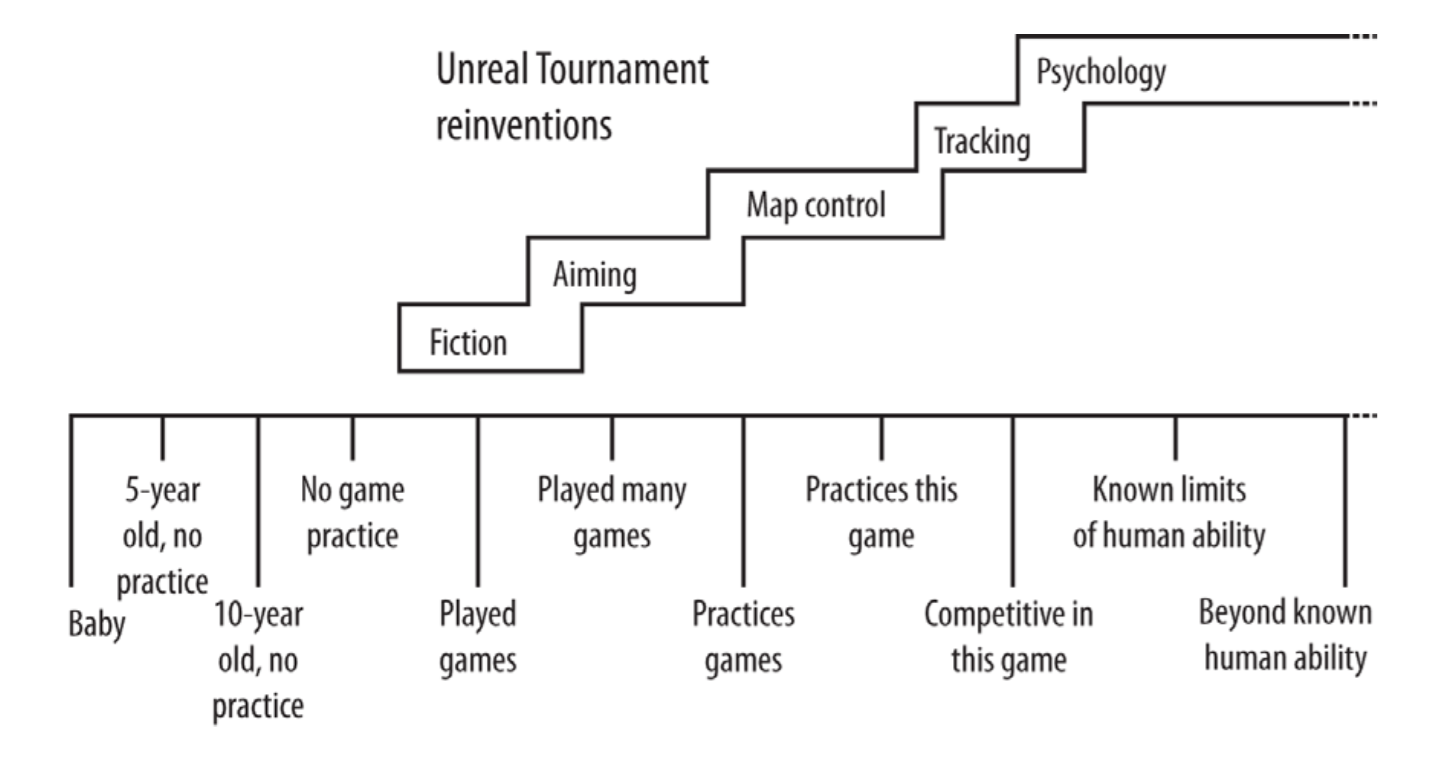
\includegraphics[width=.8\textwidth]{files/games/utSkill}
    \caption{Neuerfindung der Spielmechanik in Unreal Tournament \cite[S. 70]{Adams:1515529}}
    \label{pic:ut}
\end{figure}


Es ergeben sich drei Ebenen auf denen Neuerfindungen stattfinden können: 
%es lassen sich 3 ebnen ableiten auf denen neuerfindungen stattfinden können:
\begin{itemize}
\item Auf der Einführungsebene werden die Grundlagen für ein Spiel erlernt. Beim Schach wären dies die einzelnen Regeln, nach denen die Schachfiguren über das Spielbrett bewegt werden dürfen. So bilden die Spielregeln die Basis, auf der das Spiel aufgebaut ist.
%Dies ist die Basis auf der das eigentliche Spiel aufbaut.

\item Die Spielebene ist sehr breit. Auf ihr befinden sich die meisten Spieler. Sie kennen die Regeln des Spiels und können es ohne Schwierigkeiten bedienen. Darüber hinaus können sie ungefähr abschätzen wie sich ihre Gegner verhalten und kennen einige Strategien, um Aktionen ihres Gegenspielers zu kontern.

\item Auf der mentalen Ebene befinden sich wenige Spieler. Es gibt auch nur wenige Spiele deren Tiefgang diese Ebene erreicht. Um dieses Niveau zu erlangen muss ein Spieler sehr viel Zeit in ein Spiel investiert haben. Die größte Anstrengung für diese Spieler ist es ihre Konzentration aufrecht zu erhalten. Die Spieler auf dieser Ebene sind in der Lage Vorhersagen über Spielzüge und Aktionen im Spiel zu treffen. Auf Grund dieser Vorhersagen sind sie in der Lage Gegenspieler gezielt abzulenken bzw. zu täuschen. Jede Ablenkung und Nichtachtsamkeit kann zur Niederlage führen. Bei einem Pokerspiel beispielsweise kann das Verhalten der Spieler auf dieser Ebene beobachtet werden. So tragen einige Pokerspieler eine Sonnenbrille, um ihre Gesichtsregungen zu verschleiern. \cite[S. 71]{Adams:1515529}

\end{itemize}
%At the manual reinvention, the challenge is about simple, moment-to- moment mechanical skills. In a shooter, it is about drawing a bead on a target and holding it there. In Tetris, it is about getting pieces to fall where you want them in the rotation where you want them. In a strategy game, it is just about getting the units you want to do the thing you want them to do. In chess, it is learning how each piece can move. The manual reinven- tion is about mastering the interface. All games start here.
%The situational reinvention is the second level of skill development. At this level, manual skills are mostly unconscious. In a fighting game, the player can execute multibutton combo-strikes at will. He can aim and hit targets, or make his units move as he wants them to. The challenge at this level is not just knowing how to shoot, it is knowing who to shoot and when, or knowing what units to send and where. This is the level where most players are, and where most games are designed to function. It com- prises situational awareness, reading patterns, knowing counterstrategies, and many other midlevel game skills. This level is very broad; it can split into many internal reinventions. In my Unreal Tournament experience, both the map control and tracking reinventions were situational.
%The mental level of skill development is not reached often, and only by expert, competitive, committed players. Mental skills are all about maintaining concentration and performance. At high levels of play, an emotional upset or a momentary distraction can lead to defeat. At these heights of ability, there are tactics that are specifically about deliberately frustrating and distracting an opponent, to try to disturb his concentra- tion. Mental skill is all about predicting and manipulating his mind better than he can predict and manipulate yours. This is the pokerlike end state of most limitlessly deep games, and it is the reason most limitless games are multiplayer—because a person can learn nearly any game system, but he can never fully understand another human mind.  s. 71


\item[Flexible Herausforderungen] - Flexible Herausforderungen ermöglichen das Zusammenspiel von Spielern auf unterschiedlichen Fertigkeitsebenen. Beim Dart beispielsweise sind die Felder so angeordnet, dass auch Spieler die nicht so treffsicher sind mitspielen können. Bestünde ein Dartspiel beispielsweise nur aus dem Innenring, dem \glqq Bulls-Eye\grqq\ , wäre das Spiel für Neueinsteiger unzugänglicher, da eine sehr hohe Zielgenauigkeit vorausgesetzt würde. In Videospielen können Bewertungssysteme genutzt werden, um dieses Ziel zu erreichen. Solche Bewertungssysteme wurden schon von Spielautomaten, die in Spielhallen aufgestellt wurden, wie z.B. Flipper, eingesetzt. So ist das Spiel während des Spielverlaufs für alle Mitspieler gleich, und erst am Ende einer Spielrunde steht fest welcher Spieler wie viele Punkte erzielt hat. Indem bereits Punkte für Teilaufgaben vergeben werden, erhalten Spieler den Anreiz durch Spielwiederholungen schlechte Ergebnisse in bestimmten Bereichen zu verbessern. \cite[S. 71]{Adams:1515529}

%Ziele vergrößern und punkte vergeben. z.b. dart. es gibt nicht nur das bulls eye, es gibt zusätzlich viele felder drumherum, die getroffne werden können. so können auch spieler mitspielen, die keine profis sind. würde nur das bullseye angepasst, wäre das spiel immer für einige spieler zu einfach und für andere zu schwierig. 
%durch das einführen einer flexiblen herausforderung können alle spieler mitspielen. in vielen spielen wird daher ein highscore system verwendet. so ist das spiel für alle spieler gleich und am ende einer runde lässt sich einsehen, wie gut ein spieler abgeschnitten hat. s.71f

%Imagine a version of darts where the target is just an inch-wide bull’s-eye. Hitting the bull’s-eye gives one point, and missing it gives zero points. Such a game is so hard as to be almost pointless for anyone but experts. A designer could change the size of the bull’s-eye, but the disk will always be too small or too large for most players.
%Real darts solves this problem by wrapping concentric rings around the bull’s-eye, each of which gives a different number of points. Most people can hit the biggest ring and get a few points, but only the best can hit the bull’s-eye, so everyone has some challenging but achievable goal. This is an elastic challenge. S. 71 f
%
%
%Elastic challenges solve this problem by presenting multiple levels of success or failure. By allowing different degrees of success, they support a wider skill range since everyone has an attainable but challenging goal.
%For example, classic arcade games usually present elastic challenges using granular scoring systems. Anyone who puts a quarter in gets a few thousand points just by pushing buttons. But with enough skill and per- sistence, players can rack up hundreds of millions of points. So no matter how many times they play (and how many quarters they put in), there is always a way to do a little better.






\end{description}
%\subsection{emotional life suPPoRt} 
%\label{Abschnitt:}
%Even with good training, many players will spend the earliest parts of the game below the game’s skill barrier. For them, those first few minutes or hours become a chore to finish before the real game starts. Many will give up and never experience the game as intended.
%To stop a player from giving up before they surmount the skill barrier, we can keep their experience on life support using emotional triggers that don’t require skill.










\section{Storytelling} 
%\label{sec:}

Die Geschichte, die durch die Interaktivität eines Videospiels entsteht, wird als \glqq Emergent Story\grqq\ , zu deutsch entstehende Geschichte, bezeichnet. \cite[S. 83 ff.]{Adams:1515529} \\ 
Anders als die Ereignisse, die aus Spielmechaniken erzeugt werden, kann eine Hintergrund Geschichte für einen konstanten Fluss an Emotionen sorgen, die sog. \glqq Scripted Story\grqq\ . In diesem Punkt ähneln sich Romane, Filme und Videospiele. In der Regel findet in einem Videospiel eine Rahmenhandlung statt, die eine stringente Ordnung verfolgt. Diese Ordnung soll das Verstehen der Handlung erleichtern. In den Pausen dieser Rahmenhandlung kann ein weiterer Handlungsstrang parallel zur Haupthandlung erzählt werden. 
Zu viele dieser Nebenhandlungen können zu Verständnisproblemen führen. Anders als in Romanen und Filmen lassen sich durch die Pausen neue Spielmechaniken und Spielabschnitte (\textit{Level}) mit einzelnen Teilen der Rahmenhandlung verknüpfen. So kann beispielsweise die Suche nach einem Schlüssel, der eine bestimmte Tür öffnet, als Verbindung zwischen zwei Kapiteln der Rahmenhandlung stehen. Zusätzlich bieten sich durch die Einschnitte in der Erzählung Gelegenheiten in denen der Spieler sich mit neuen Spielmechaniken vertraut machen kann. Er kann die Mechaniken lernen und eintrainieren, ohne dass er der Handlung folgen muss. Neue Spielmechaniken wirken bedeutungsvoller, wenn sie zu Beginn einer neuen Storyline eingeführt werden. Etwas neu erlerntes direkt wieder in einem neuen Kontext zu verwenden verstärkt die Emotionen.
\cite[S. 96]{Adams:1515529}\\
%Dieses Prinzip kann an vielen Stellen in Spielen verwendet werden. So können mit diesen Handlungen Geschichten parallel zum Haupthandlungsstrang erzählt werden. 
%Spielmechaniken parallel zu einer neuen storyline einführen
%Ordnung von Storyelementen:
%Level, Quests (mini story), Blockierung ( Tür>Schlüssel finden, Level) kann auch nicht konsequent durch gesetzt werden und aufgaben freier gestalten, skillgating gehört auch dazu 
%viele weitere oft wird auch Zeit genutzt, npcs zu bestimmten uhrzeiten,
%Most story media are restricted to a small set of tools. A comic book storyteller gets written speech bubbles and four-color art. A filmmaker gets 24 frames per second and stereo sound. A novelist gets 90,000 words. A museum exhibitor gets the layout of the space, info panels, dioramas, and perhaps a few interactive toys.
%Games are broader. Like film, we can use predefined sequences of images and sounds. Like a novel, we can use written text. Like a comic book, we can put up art and let people flip through it. Like a museum, we can create a space for players to explore. And we have tools that nobody else has: we can create mechanics that generate plot, character, and even theme on the fly, and do it in response to players’ decisions.
%Überleitung Mechanik > Story
%During any play session, game mechanics, players, and chance come to- gether to create an original sequence of related events which constitute an emergent story.
%EMERGENT STORY is story that is generated during play by the interaction of game mechanics and players.
%When you play a racing game against a friend and come back to win after a bad crash, that’s a story. But it wasn’t written by the game de- signer—it emerged during your particular play session. This is emergent story. S.90
Der Verlauf der Geschichten ist trotz Unterbrechungen linear. Die Linearität liegt im festen Handlungsablauf, auf den der Leser bzw. Zuschauer keinen Einfluss hat. Filme und Romane bieten keine Interaktivität oder Auswahlmöglichkeiten.
%, sind keine präsenz(zeit) erfahrung
Museen und Kunstgalerien sind interaktiv. Der Besucher hat selbst die Möglichkeit zu entscheiden in welcher Reihenfolge er die Ausstellungsstücke betrachtet. Durch Schilder und Hinweise kann der Betrachter in bestimmte Richtungen gelenkt werden, muss diese aber nicht zwingend einhalten. Ähnlich ist es mit dem Tatort eines Verbrechens. Die ermittelnden Polizisten müssen aus den einzelnen Details, die sie dort vorfinden, auf den Tathergang schließen.  \cite[S. 82]{Adams:1515529}
Neben diesen Entscheidungsmöglichkeiten beeinflusst auch die Umgebung die gesamte Handlung. Ein Betrachter einer Szene entwickelt eine Geschichte auf Grund der Eindrücke die er durch die Umgebung erhält. Eine verwüstete Stadt kann so beispielsweise wie ein Kriegsschauplatz wirken. Durch Änderungen an diesem Bild, kann es auch so auf den Betrachter wirken, als sei die Stadt durch eine Naturkatastrophe zerstört worden. Eine dritte Variante wäre, dass die Stadt verlassen worden ist und die Häuser im Laufe der Zeit verfallen sind. Diese Erzählweise wird als \glqq World Narrative\grqq\ bezeichnet. \cite[S. 86 f.]{Adams:1515529}\\
Es ergeben sich somit drei Erzählweisen für die Geschichte eines Spiels:
\begin{itemize}
\item Die fest geschriebene Geschichte, die \glqq Scripted Story\grqq\ .
\item Die sich aus den Ereignissen des Spielverlaufs ergebende Geschichte, die \glqq Emergent Story\grqq\ .
\item Die durch die Umgebung erzeugte Geschichte, die \glqq World Narrative\grqq\ .
\end{itemize}

Auf diese drei Bereiche können die Spielmechaniken Einfluss nehmen. Sie können die Handlung des Spiels beeinflussen, zu einer Charakterentwicklung führen und auch die Szenerie augenblicklich ändern. So kann ein Spieler direkten Einfluss auf die gesamte Story ausüben. Dies ermöglicht nicht nur lineare Erzählstrukturen. Hier werden die Unterschiede zwischen Videospielen und anderen Medien besonders deutlich. 
%wobei diese anderen mit den Entscheidungen des spielers verknüpft sind.
%dies zeigt, wie stark die Erzählweise in spielen von den herkömmlichen abweicht.
%so lässt sich an dieser stelle die Erzählweisen in drei Bereiche zusammenfassen. der scripted story, also der zu vor festgesetzten Geschichte, der World narrative, der Geschichte die eine Szene von sich erzählt und der exklusiv den Videospielen zugehörigen emergent story, eine Geschichte, die zur Laufzeit des Spieles entsteht.
%nichtlinear bei denen der besucher zwar in eine richtung gelenkt wird aber sie dennnoch auf seine eigene art durchläuft. bei ruinen und grafties ist das ähnlich. 
%aber auch der tatort eines verbrechens kann als eine interaktive erzählung sein. so muss der ermittelnde polizist aus den einzelnen details wie blutspuren und zerbrochenem glas schließen, was vorgefallen ist. s.82 f
%A completely free-form game would allow the player to take any path through its narrative content. Imagine tearing out all the pages of a novel and scattering them all over the floor. One could lean over and read any page, switch to another page, and to another, navigating randomly through the text. That’s a narrative with no ordering at all, since the reader can absorb the content in any order. 
%A story can work like this, to an extent, as in the earlier example of world narrative. But most narrative tools still work better when we control the order in which they’re used. Sometimes we want to ensure the setup occurs before the payoff. We might want to let one subplot play out before we add another so we don’t have too many plot threads running at once. Or perhaps we want to introduce game mechanics one by one alongside the story so we can train the player in a smooth progression. In each case, we need some way to make sure one piece of content is consumed before another.
%Games use a variety of devices to enforce story ordering:
%Levels are the classic story-ordering device. Players play the first level to completion, then the second, then the third, and so on. It’s old, it’s simple, and it works.
%Quests are another classic story-ordering device. A quest is a self- contained mini-story embedded in a larger, unordered world. The world might span an entire continent while a quest might cover the player help- ing one shopkeeper rid himself of an extortionist. The quest starts when the player meets the shopkeeper and hears his plight. The player then finds the mobster, convinces him to stop or beats him up, and finally re- turns to the shopkeeper to get paid. Within this sequence, the order of events is fixed. But this mini-story could be started and finished at any time as the player explores the city. And it can be suspended: the player might meet the shopkeeper, beat up the mobster, then get distracted and go slay a dragon in another part of the world before finally returning to the shopkeeper to get his reward.
%A third basic story-ordering device is the blockage. The simplest block- age is a locked door. The player encounters the door, and he must go find the key before progressing. So whatever happens while he’s acquiring the key is guaranteed to occur before whatever happens beyond the door. Blockages don’t have to literally be locked doors either; perhaps a guard won’t let you past until you go do him a favor, or a security camera will spot and stop you unless you first go turn off the lights.
%There are also softer story-ordering devices. These devices encourage an order to the story without absolutely guaranteeing it.
%Skill gating is a soft story-ordering device. With skill gating, players can access all the content in the game from the first moment of play. However, some of the content requires the player to exercise skill before it can be accessed. To talk to a character, for example, the player might first have to defeat him in combat. Players end up experiencing the content in rough order as they progress along the skill range, even though all the content is technically available from the start.
%A version of skill gating is used in many massively multiplayer RPGs. The player can technically go anywhere from the start, except that he doesn’t have the skill, character upgrades, or allies necessary to survive far outside his starting area. So the game has the feeling of a massive open world, while still gently directing new players through a carefully designed sequence of introductory challenges.
%There are countless other kinds of story-ordering devices. Time-based games like Dead Rising make events occur in the world on the clock at fixed times. A quest might open up when the player character reaches a certain level of progression. Even simple arrangements of space can create a soft story ordering, as players are likely to encounter the nearby pieces before the more distant ones.
%Parallelen zwischen Film und Videospielen, bewegtes Bild und Ton
%Aber Spiele funktionieren anders
%die meisen medien haben nur wenig werkzeuge.
%comicbuch hat sprechblasen und bilder, ein kinofilm hat 24 fps und verschiedene audiospuren. ein romanautor eine bestimmte anzahl an worten. ein aussteller in einem museum erhält seinen zugewiesenen platz mit dem zugehörigen layout, info panäle und evtl ein diorama und oder ein paar interaktive spielereinen.
%spiele decken einen größeren Bereich ab. sie bieten die Fähigkeiten von bewegten Bildern und sounds, können zudem aber noch Texte wie in einem buch oder in einer Sprechblase, wie in einem comic, wiedergeben. der Nutzer hat dabei sogar die Möglichkeit ganze Kapitel oder Seiten zu überspringen. es können aber auch wie im museum bereiche definiert werden, an denen der spieler die geschichte selbst erkundet. hinzu kommen weitere Werkzeuge, die im keinen der zuvor genannten Medien vorhanden sind. 
%The advantage of this soft-scripted approach is that it doesn’t break flow since the player’s controls remain uninterrupted. The downside is the control it takes away from the designer. The player might be able to watch the murder from an ugly angle, miss it entirely, or even interfere with it.
%For example, a hint might require enemies to stay in the rear half of a room, but still allow them to autonomously shoot, grab cover, dodge grenades, and punch players who get too close. Designers use these hints to author higher-level strategic movements, while the AI handles moment-by-moment tactical responses to player behavior.
%
%There are also ways of scripting events which are naturally immune to interference. Mail can arrive in the player character’s mailbox at a certain time. Objects or characters can appear or disappear while the player is in another room. Radio messages and loudspeaker broadcasts can play. These methods are popular because they are powerful, cheap, and don’t require the careful bespoke design of a custom semi-interactive scripted sequence.
%
%All places tell stories. We can explore any space and discover its people and its history. Game designers can use this to tell a story by embedding it in a space. I call this world narrative.
%
%Next, world narrative does not need to be told in linear order. This saves us from having to railroad players into a specific path. For example, imagine that the narrative content is that two lovers fought, and one mur- dered the other and buried him in the backyard. Told through the world narrative a day later, it doesn’t matter if the player discovers the corpse or the bloody bedroom first. As long as he sees both, in either order, he will be able to piece together what happened. This means that a game de- signer can let the player explore the house freely. Telling the same story in scripted events would require that the designer come up with some trick or restriction to ensure players follow the right path through the space in order to see all the events in the right order.
%
%
%World narrative’s last great advantage is that it supports players re- playing the game because it doesn’t always reveal itself completely the first time around. Whereas scripted stories uncover themselves event by event from start to finish, world narrative naturally uncovers itself in order
%
%
%When you play a racing game against a friend and come back to win after a bad crash, that’s a story. But it wasn’t written by the game de- signer—it emerged during your particular play session. This is emergent story.
%We can look at emergent story in two ways: as a narrative tool, and as a technology for generating story content.
%
%Showing and telling players less creates more room for apophenia to fill in the gaps.
%
%More detailed graphics and higher-quality sound add something to a game, but they also take something away. The more detailed the graphics, sound, and dialogue of a game, the less space there is for interpretation.The more abstract, nonspecific, and minimalistic the representation, the more apophenia becomes possible.
%
%
%
%But most narrative tools still work better when we control the order in which they’re used. Sometimes we want to ensure the setup occurs before the payoff. We might want to let one subplot play out before we add another so we don’t have too many plot threads running at once.
%
%
%
%Or perhaps we want to introduce game mechanics one by one alongside the story so we can train the player in a smooth progression. In each case, we need some way to make sure one piece of content is consumed before another.
%
%
%Quests    blockage     Skill gating 
%
%..
%This book won’t discuss what makes a good story. Better authors than I have been covering this topic ever since Aristotle wrote his Poetics. They’ve already explained how to craft a plot with interesting reversals and good pacing. They’ve described how to create lifelike, layered characters who are worth caring about. They’ve explored theme, setting, and genre. I’m not a dedicated story crafter; I doubt I have much to add to this massive body of knowledge (though game designers should understand these ideas, so I’ve recommended a starting text at the end of the book). 
%\section{Erzählstrukturen in Videospielen} 
%\label{sec:}
\pagebreak

Das Zusammenspiel der Elemente, die eine zusammenhängende Geschichte erzeugen können, bieten in einem Videospiel mehrere Möglichkeiten eine Geschichte zu strukturieren. Zusätzlich zur schriftlichen Beschreibung der Strukturen folgen Abbildungen (\ref{pic:storyLinear} bis \ref{pic:storyHybrid}) in denen die beschriebenen Strukturen bildlich dargestellt werden. Kreise stehen für Storyabschnitte und Pfeile stehen für eine Überleitung, durch die ein Spieler durch die Geschichte eines Spiels geführt wird.

\begin{description} 
\item[Lineare Erzählung]  - Diese Erzählweise spiegelt ein Buch oder einen Film wieder. Übertragen auf ein Spiel heißt das, der Spieler wird mit jedem Level einen Schritt weiter durch die Story geführt. Dabei muss der Umfang der Storyelemente beachtet werden. Das Spielen von kurzen Levels mit wenig Hintergrundgeschichte kann dazu frühen, dass das Spiel keine Spannungsspitzen erreicht. Diese Erzählweise wird in Abbildung \ref{pic:storyLinear} dargestellt. %Dieses Erzählweise wurde z.B. in den klassischen Super Mario Bros. Spielen aber auch in einigen anderen Spielen, wie z.B Quake oder Stracraft, verwendet. 
\cite[S. 98]{Adams:1515529}


\begin{figure}[H]
    \centering
    
\includegraphics[width=.8\textwidth]{files/story/storyLinear}
    \caption{Veranschaulichung der linearen Struktur \cite[S. 98]{Adams:1515529}}
    \label{pic:storyLinear}
\end{figure}
 
\item[Geschichte mit zentralem Knotenpunkt] 
Bei dem zentralen Knotenpunkt steht ein Level oder ein spielbarer Bereich im Mittelpunkt. Mit ihm sind alle anderen Elemente verbunden. Dem Spieler steht so beispielsweise eine Basis zur Verfügung, von der er die Geschichten der anderen Level in beliebiger Reihenfolge erleben kann. Dies Erzählstruktur kann auch in erweiterter Form auftreten, bei der ein Spieler erst einige Level gespielt haben muss, um weitere Level freizuschalten. So kann der Spieler in einem gewissen Maß selber festlegen, wie die Story voranschreitet. \cite[S. 98f.]{Adams:1515529} \\
%Die basis Version hiervon ist in den Megaman Spielen zu finden. Dort kann der Spieler in einer Art Menü auswählen, welches Level er als nächstes spielen möchte. 
Im Spiel \glqq Super Mario 64\grqq\ ist eine erweiterte Version dieses Modells realisiert. Der Spieler bewegt sich in einem Schloss und hat die Möglichkeit verschiedene Level zu spielen. Es ist ihm aber nicht möglich von Anfang an alle Level zu betreten. Einige Level sind versteckt und müssen erst vom Spieler entdeckt werden, andere benötigen einen gewissen Fortschritt im Spiel.\\ %Nicht alle Level müssen gespielt werden, um die Hauptgeschichte des Spiels abzuschließen.
In der Abbildung \ref{pic:storyKnoten} wird die Grundversion dieser Erzählstruktur dargestellt.


\begin{figure}[H]
    \centering
    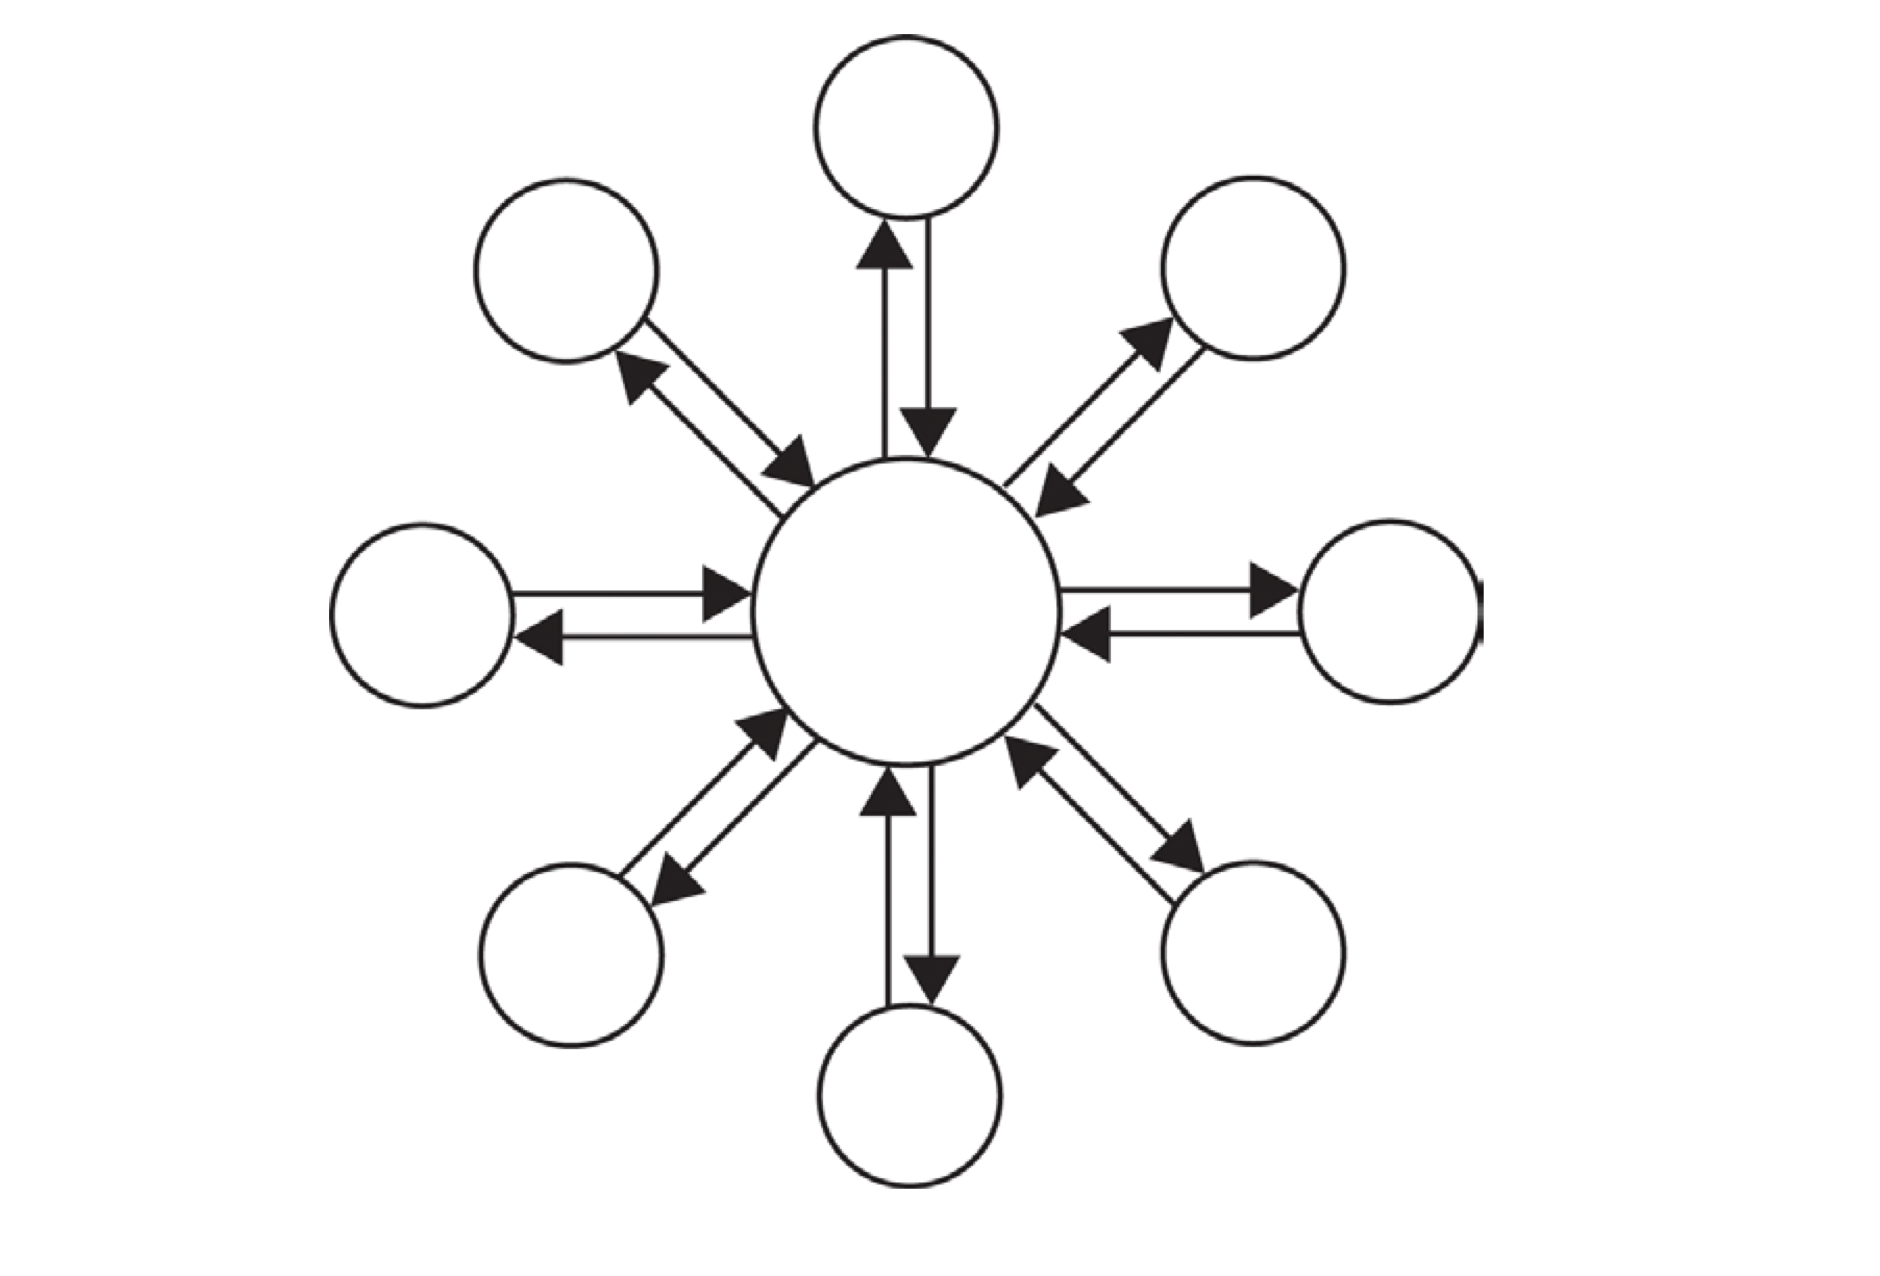
\includegraphics[width=.8\textwidth]{files/story/storyZentralKnoten}
    \caption{Veranschaulichung des zentralen Knotenpunkt \cite[S. 98]{Adams:1515529}}
    \label{pic:storyKnoten}
\end{figure}


 
\item[Komplett entscheidungsgesteuerte Geschichte]

Diese Erzählstruktur ist an das reale Leben angelehnt. Der Spieler hat nach jedem Abschnitt im Spiel die Wahl, wie er weiter in der Geschichte des Spiels voranschreiten möchte. Durch die Entscheidungsmöglichkeiten entstehen neue Verzweigungen in der Geschichte. Dadurch wächst die Anzahl der Storyelemente bzw. Levels exponentiell. Es werden daher viele Abschnitte für ein Spiel benötigt, die von einem Spieler nicht erlebt werden können. Es müssen viele Abschnitte entwickelt werden, die später vom Spieler in der Regel nicht gespielt werden. In Abbildung \ref{pic:storyEntscheidung} wird dieser Ansatz bildlich dargestellt. Im abgebildeten Beispiel stehen dem Spieler in jedem Abschnitt zwei unterschiedliche Auswahlmöglichkeiten zur Verfügung. Für sechs Situationen in denen ein Spieler eine Entscheidungsmöglichkeit hat, würden so 127 einzelne Storyabschnitte benötigt. \cite[S. 99]{Adams:1515529} 
%Spielern wird viel vorenthalten. 


 
\begin{figure}[H]
    \centering
    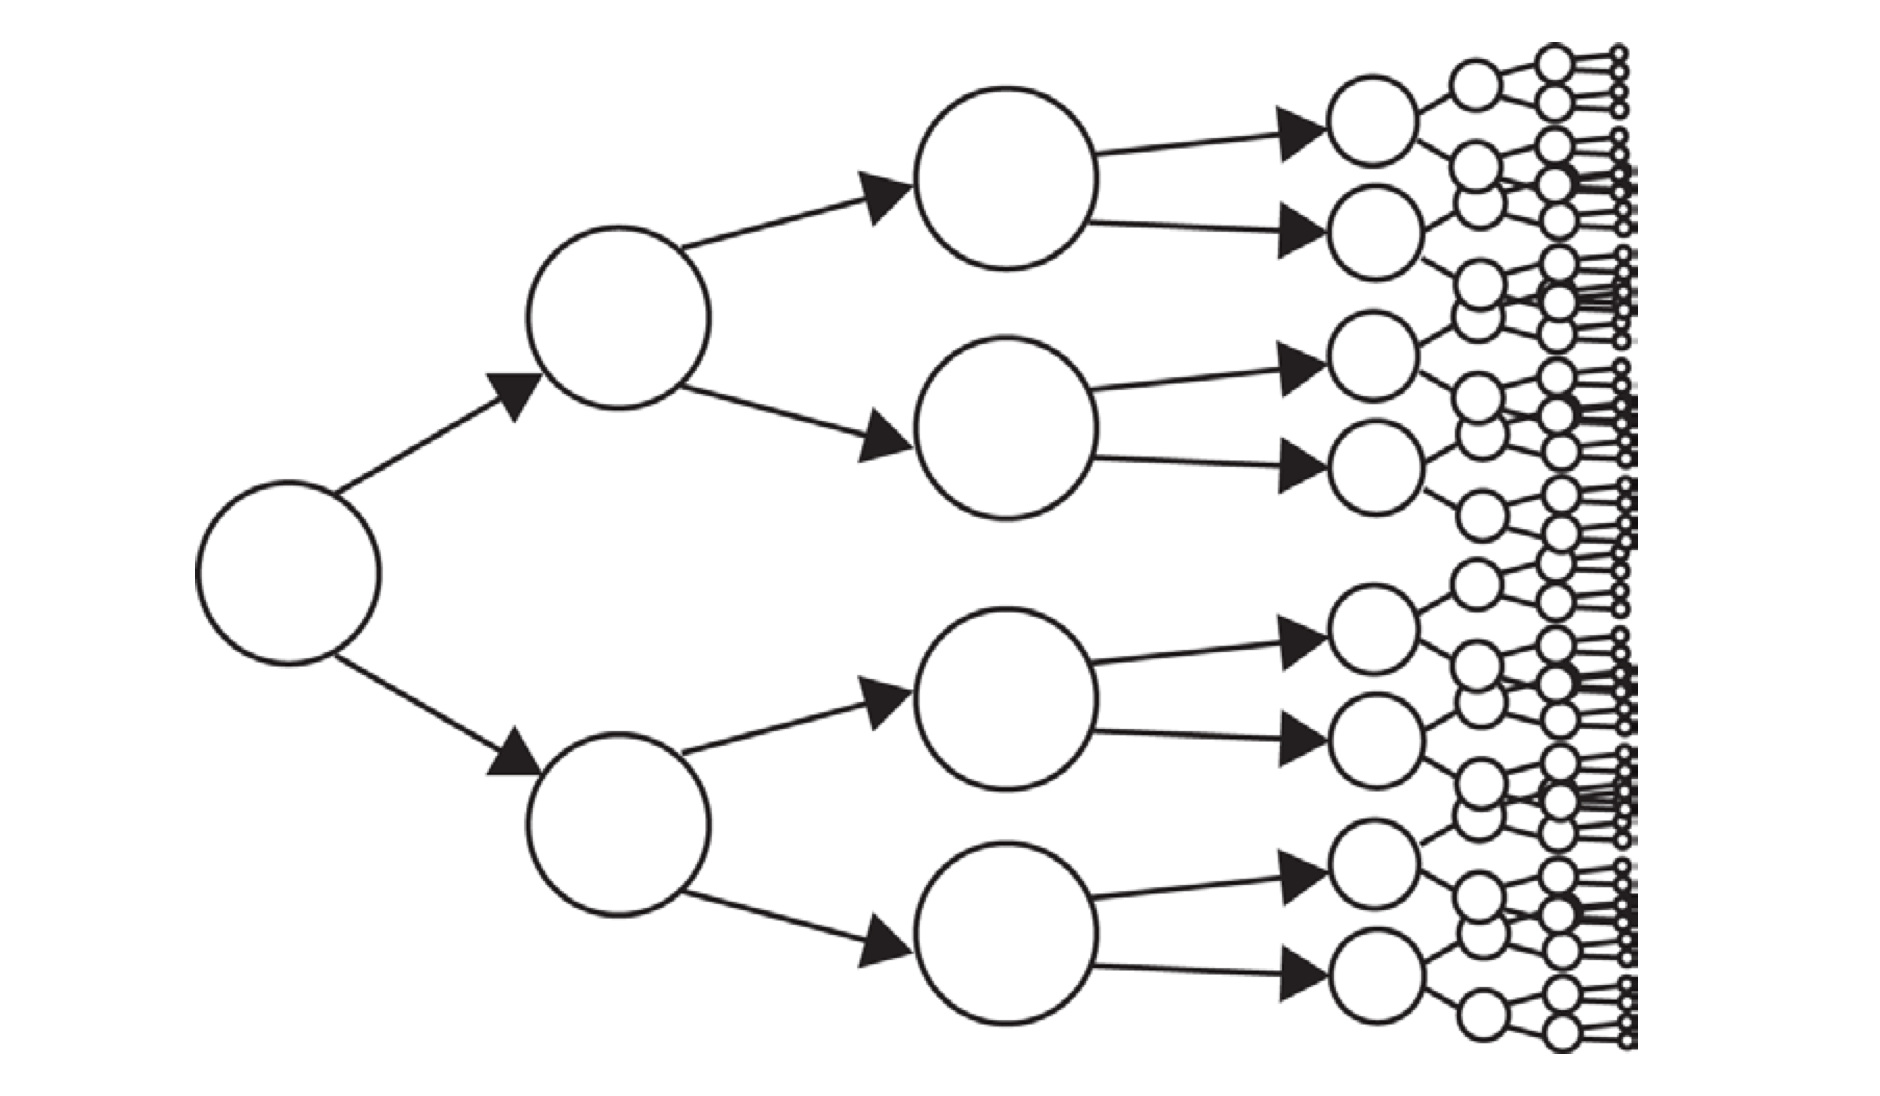
\includegraphics[width=.8\textwidth]{files/story/storyEntscheidungen}
    \caption{Veranschaulichung der komplett Entscheidungsgesteuerten Variante}
    \label{pic:storyEntscheidung}
\end{figure} 


\item[Nicht lineare Geschichte mit optionalen Abschnitten]
Diese Erzählstruktur vereint den linearen mit dem entscheidungsgesteuerten Ansatz. Es kann in einem Spieldurchlauf nicht die gesamte Hintergrundgeschichte vom Spieler erlebt werden. Durch sog. \glqq Sidequests\grqq\ (Nebenhandlungen), die an einzelne Abschnitte angehangen werden können, kann ein Spieler optionale Storybestandteile erfahren. \glqq Sidequests\grqq\ müssen vom Spieler nicht gespielt werden. Sie können beispielsweise den Hintergrund eines Spielcharakters genauer erläutern. Durch den Einsatz von Entscheidungen, die einen direkten Einfluss auf den Verlauf der Spielgeschichte haben, wird ein Spieler indirekt mit in die Geschichte einbezogen. Dies hat zur Folge, das er die Geschichte intensiver wahrnimmt. In der Abbildung \ref{pic:storySQ}
wird diese Struktur mit einem \glqq Sidequests\grqq\ und einer Entscheidung dargestellt. Bei nur einem Spieldurchlauf würde der Spieler so mindestens einen Abschnitt nicht erleben können. \cite[S. 100]{Adams:1515529}
%, die vom Spieler nicht gespielt werden müssen. \glqq Sidequests\grqq\ können die
% Es ist möglich nicht die ganze Story zu erleben
%Ein Teil der Story ist abgekapselt
%Haupstory verläuft zum Linear, kleine Exkursion
\begin{figure}[H]
    \centering
    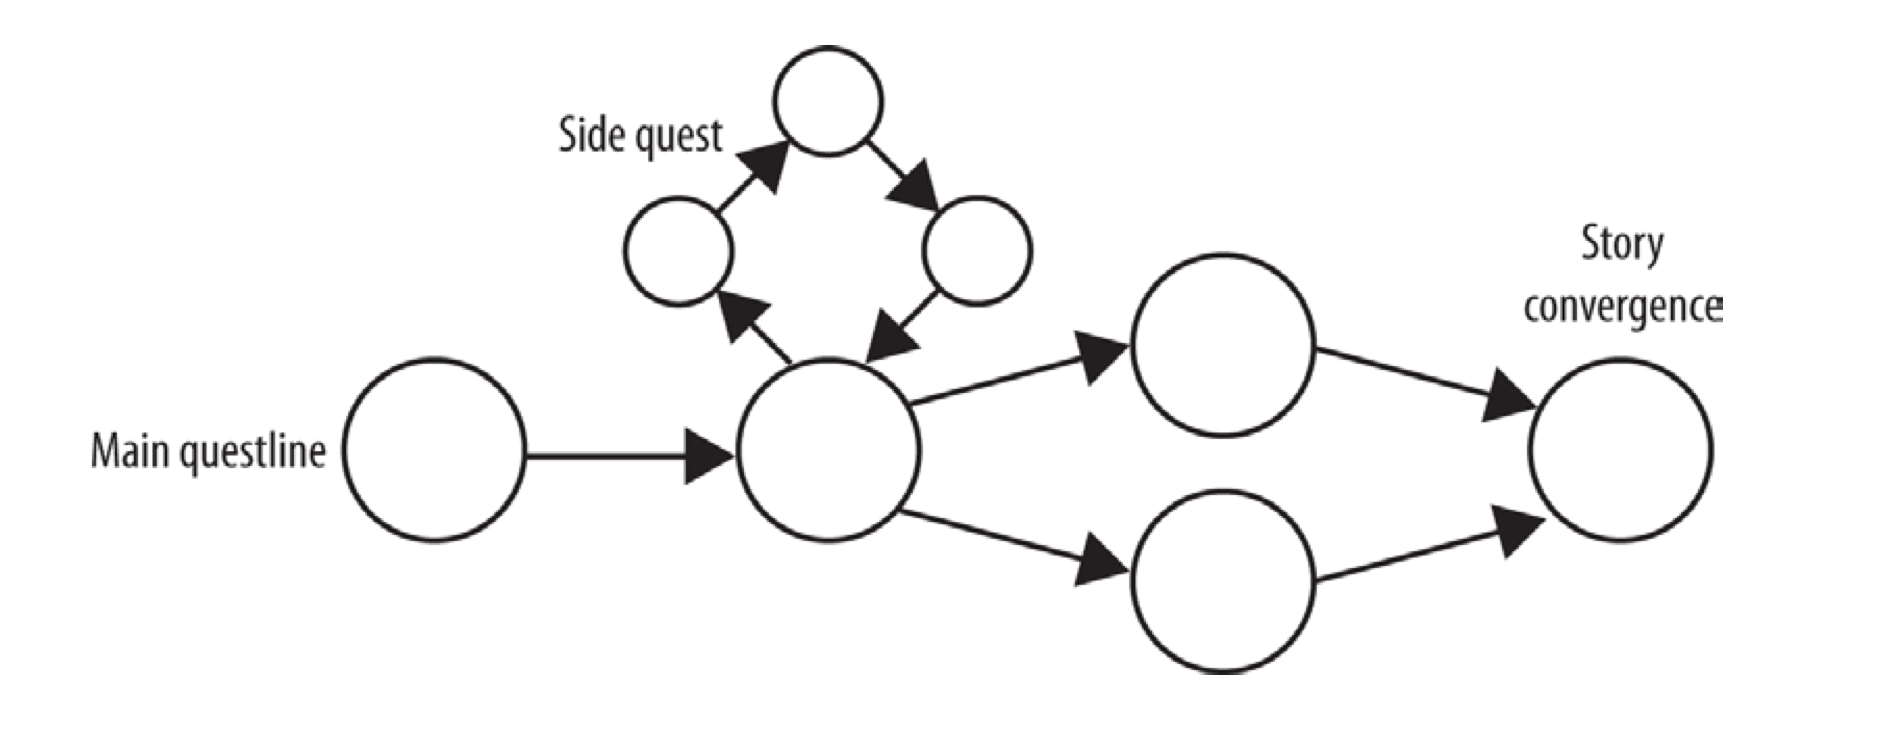
\includegraphics[width=.8\textwidth]{files/story/storySidequest}
    \caption{Veranschaulichung der nicht linearen Story mit Sidequest}
    \label{pic:storySQ}
\end{figure} 

%\item[Zentraler Knotenpunkt mit linearem Fortsatz]
%
%Ähnlich wie oben, aber nachdem die ersten Storyteile gespielt wurden
%Wird linear fortgesetzt
%\cite[S. 100]{Adams:1515529}
%Abbildung \ref{pic:storyKnotenPlus}
%
%
%\begin{figure}[H]
%    \centering
%    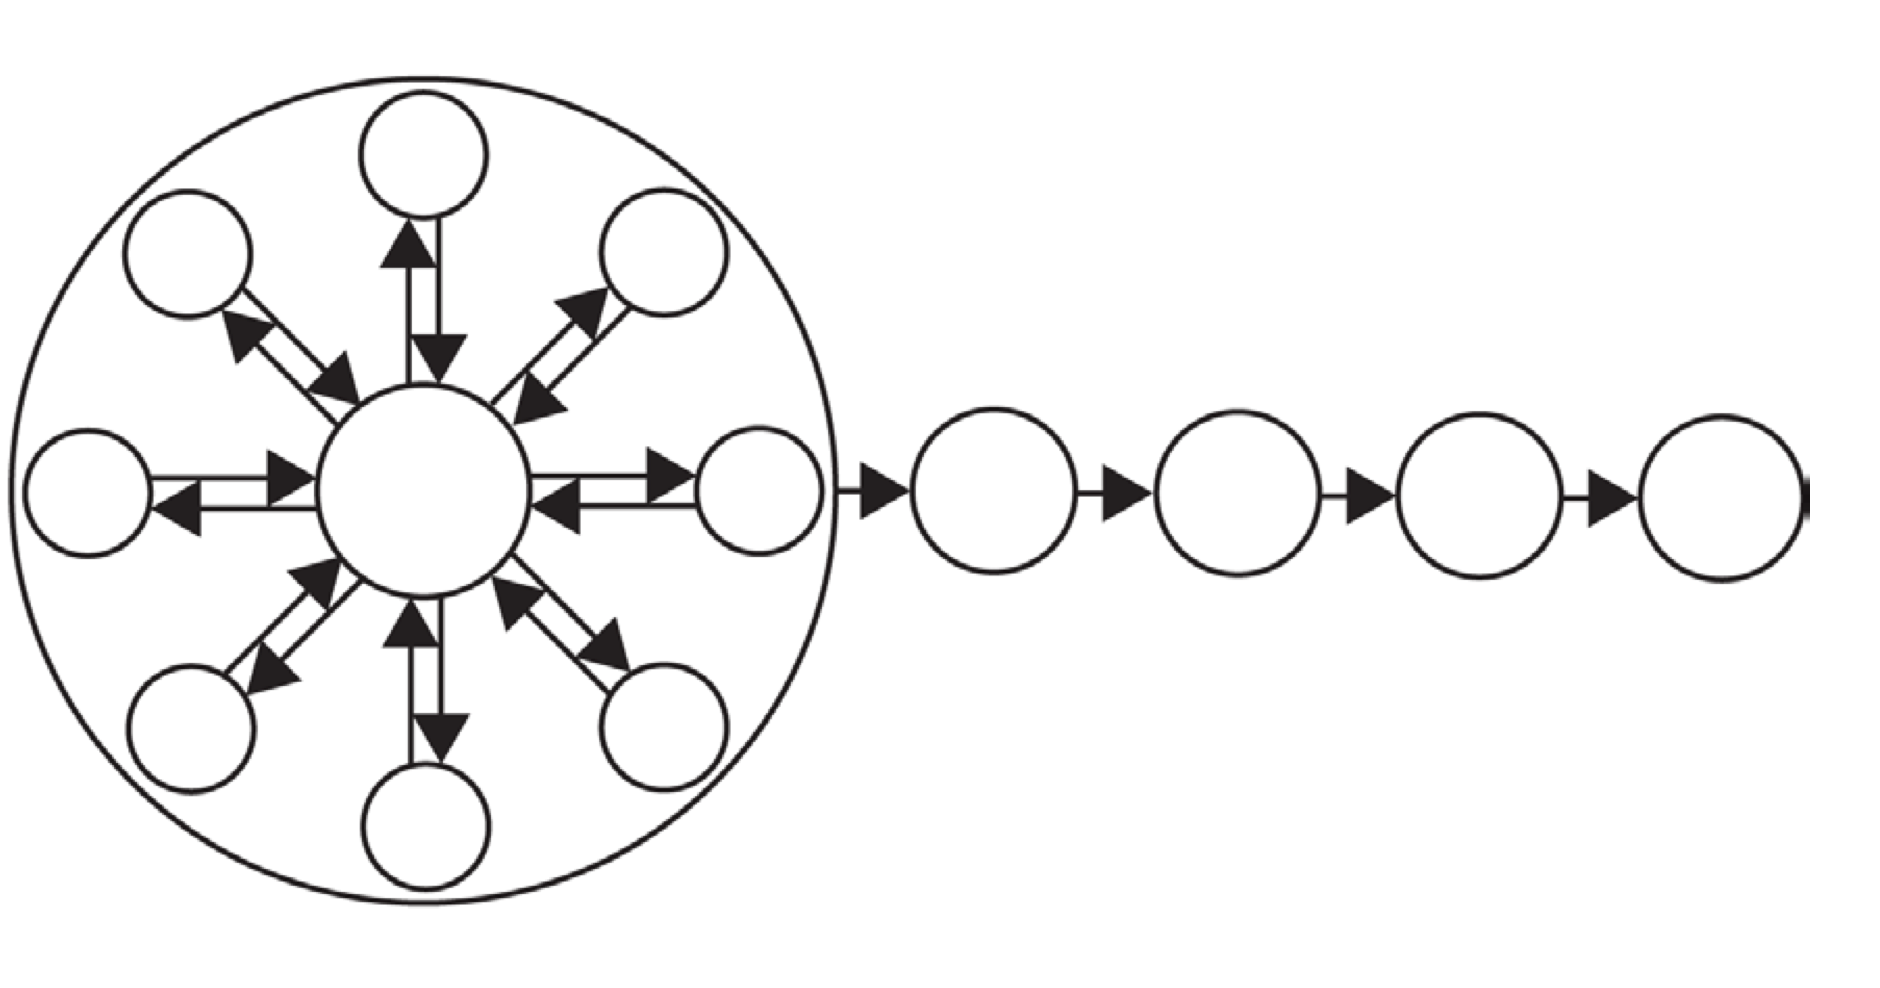
\includegraphics[width=.8\textwidth]{files/story/storyZentralKnotenLinear}
%    \caption{Veranschaulichung des zentralen Knotenpunkts mit linearem Fortsatz}
%    \label{pic:storyKnotenPlus}
%\end{figure} 


\item[Hybride Erzählstruktur]
Der hybride Storyansatz verbindet die vorherigen Ansätze miteinander. In der Spielwelt gibt es verschiede Erzählstränge, die frei vom Spieler gewählt werden können. Dem Spieler wird keine Reihenfolge vorgeschrieben, in der er die einzelnen kleinen Geschichten spielen soll. Diese kleinen Geschichten bzw. Episoden können zur Hauptgeschichte betragen, müssen es aber nicht. \\
In der Abbildung \ref{pic:storyHybrid} wird ein hybrider Ansatz dargestellt mit einem linearen Anfang und einem linearen Ende. Dazwischen befinden sich einzelne, zum Teil verkettete Storyelemente, die in beliebiger Reihenfolge gespielt werden können.
 
%Linear mit teilweise verketteten Storytelementen
%Anfang und Ende sind linear
%Flickenmuster aus Sidequests, die zur hauptgeschichte beitragen
%Spieler kann entscheiden, was er erleben möchte.
%Kann die Geschichte auch beenden ohne alle Informationen gesammelt zu haben. \\
\cite[S. 100 f.]{Adams:1515529}


\begin{figure}[H]
    \centering
    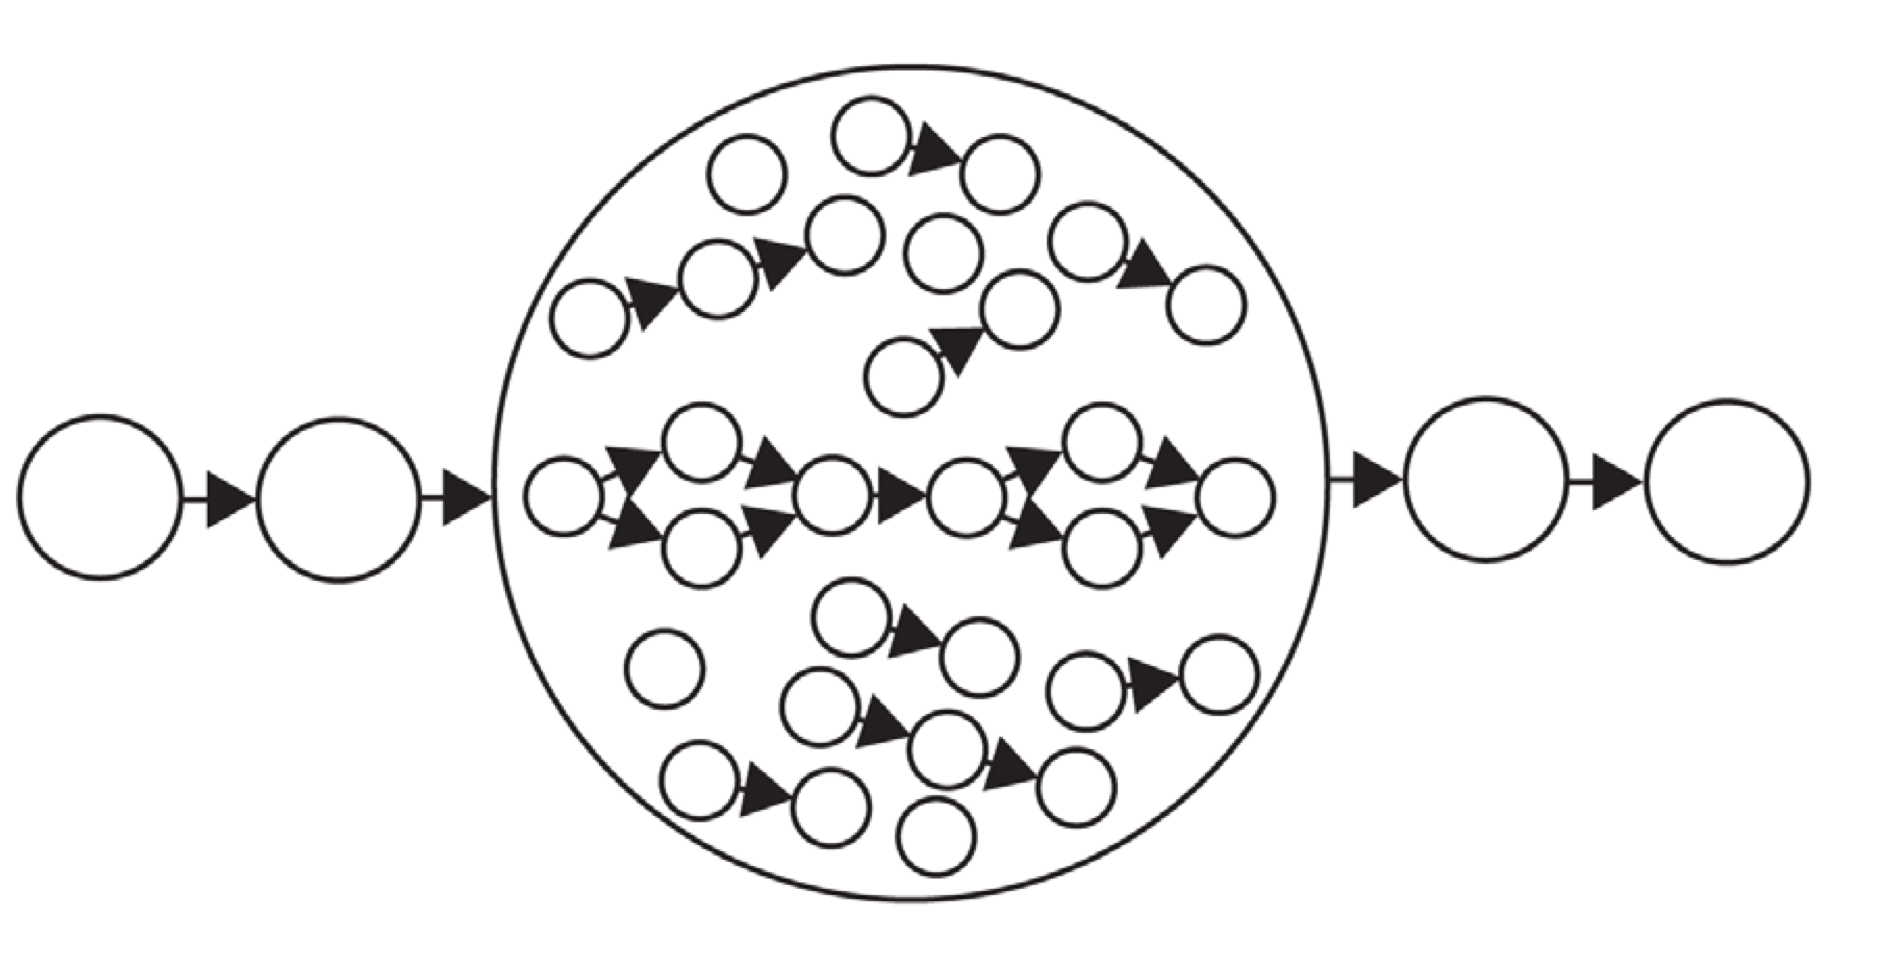
\includegraphics[width=.8\textwidth]{files/story/storyTeile}
    \caption{Veranschaulichung des hybriden Ansatzes}
    \label{pic:storyHybrid}
\end{figure} 


%\cite[Seite 12]{Adams:1515529}







\end{description}

\pagebreak

Die vorgestellten Erzählstrukturen lassen sich durch \glqq Cutscenes\grqq\, zu deutsch, Zwischensequenzen unterteilen. In diesen Szenen stehen dem Entwickler oder Storywriter alle Tricks des Films zur Verfügung. Es können z.B. Zeitlupeneffekte, Schnelldurchläufe und Nahaufnahmen von Protagonisten gezeigt werden. Darüber hinaus gibt es viele weitere dramaturgische Techniken eine Szene aufzuwerten. \glqq Cutscenes\grqq\ werden in der Regel dazu genutzt die Geschichte eines Videopiels voranzutreiben. Der Einsatz des Hilfsmittel führt zu harten Übergängen, da dem Spieler die Kontrolle und somit der Einfluss auf diese Szenen entzogen wird. Richtig eingesetzt können sie eine gute Trennung von Spielabschnitten sein. Sie können als eine Art der Belohnung für das Erreichen eines Spielabschnittes benutzt werden. \\
%Zwischen verschiedenen Kapiteln der Geschichte des Spiels können sie störend wirken.  \\
Im Spiel \glqq Tetris\grqq\ für den Gameboy beispielsweise, wird nach Beendigung einer Spielrunde und ab dem Überschreiten einer Mindestpunktzahl ein Video angezeigt. Je nach Höhe des Punktestandes der Runde wird der Start unterschiedlicher Raketen dargestellt.  \\
%Diese bringen aber immer einen harten Übergang mit sich, denn dem Spieler wird die Kontrolle über das Spiel entzogen. Werden Cutscenes zu häufig eingesetzt, wird der Ablauf des Spiels zu einem stop-start Erlebnis und somit abgehackt wirken. Richtig eingesetzt, können sie aber eine gute Trennung von Spielabschnitten darstellen. Trotzdem sind die cutscenes immer ein holpriger Übergang. 
Um den Übergang zwischen einer \glqq Cutszene\grqq\ und dem Spiel fließender zu gestalten, gibt es den sog. \glqq soft-scripted\grqq\ Ansatz. Bei diesem Ansatz behält Spieler die Kontrolle. Er kann also z.B. seinen Charakter weiter steuern. Hierdurch verliert der Designer jedoch einen Großteil der Kontrolle über die Szene. Das kann verschiedene Nachteile mit sich bringen. Ein Spieler könnte beispielsweise die jeweilige Szene aus einem ungünstigen Blickwinkel oder ggf. gar nicht erleben. Es wäre auch denkbar, dass der Spieler versucht eine Interaktion durchzuführen, die nicht vorgesehen ist und so beispielsweise einen verbündeten Charakter erschießt. So können Fehler im Handlungsstrang entstehen, die im weiteren Verlauf der Geschichte nicht korrigiert werden können. 


%In einem Spiel mit Charakteren in der Rahmenhandlung, sollte stets versucht werden die Ziele des gespielten Charakters auf den jeweiligen Spieler zu projizieren.



 
%PlayeR–CHaRaCteR motivation alignment
%Many agency problems appear because the player’s motivations are differ- ent from those of the character he controls.


%DESK JUMPING is when the player takes an action that the player character would never take because their motivations are different.
 
%Sometimes we can incorporate the desk jumping into the narrative.


%Traditional stories are built from character interaction. Characters betray, demand, suggest, declare, debate, and dialogue their way through a series of emotional turns that constitute a story. This applies to nearly all stories, not just dramas. Even the most pyrotechnic of action films and the bloodi- est of horror stories fill most of their time with people talking.
%This is a problem for game designers, since there is currently no way to do rich human interaction with a computer. Buttons, joysticks, and simple motion sensors aren’t enough to allow people to express thoughts and feelings to a machine. Furthermore, even if players could express themselves to the machine, the machine would not be able to respond in kind because we have no technology that can simulate a human mind.
%To make human interaction work in games, we can use a set of tricks that get around the limitations of the medium.
%We can set up the fiction so that there is naturally no way to interact directly with humanlike characters.


%In BioShock, for example, sane characters only ever speak to the player over a radio or through unbreakable glass. The characters who can be con- fronted face to face are all violently insane. You can watch these madmen as they go about their broken lives and listen to their deranged muttering, but this works because you’re not interacting, just watching as they follow a predefined script. As soon as you try to interact, they fly into a murderous rage that the computer can simulate without trouble.
%DIALOGUE TREES can handle human interaction by predefining a list of actions players can take and matching responses from other characters. 



\section{Ortung/Ortsbezug} 
\label{Abschnitt:}




%\section{Grundlegende Gedanken zur Spielmechanik}
%\label{sec:}
%Der wichtigste und zugleich grundlegende Gedanke ist, wie andere Menschen dazu gebracht werden können Zeit in ein Spiel zu investieren. Dazu wird zunächst ein Blick in die Psyche der Menschen geworfen um zu entscheiden, was als Aspekt dienen kann. Das Spielen in der Kindheit ist eine Art lernen erwachsen zu sein. Ein blick in den Kindergarten zeigt, dass die meisten Kinder Fangspiele spielen oder bauen, z.B. im Sandkasten oder mit Bausteinen. Bei Jungen kommt es auch des Öfteren zu Kämpfen untereinander. \\
%Alle Kinder spielen diese Spiele. Nicht nur ein- oder zehnmal, sondern jeden Tag und warum werden sie es nicht leid diese Spiele zu spielen.
%Der wichtigste Punkt ist gewinnen macht Spaß. Jedoch darf die Herausforderung nicht fehlen. Genau dies ist es was die Kinder beim Spielen hält. Beim fangen, sowie beim Kämpfen werden auch die anderen Kinder immer geschickter, können besser ausweichen, werden schneller beim laufen. Beim Bauen müssen die Türme höher und stabiler werden. Trotzdem kann so etwas auch irgendwann langweilig werden, wenn jemand so viel besser als die anderen sind, dass keiner mehr mit ihm spielen will.\\
%
%- Urtriebe\\
%- Traning erwachsen zu sein \\
%- nicht genau das was Videospiele sind \\


%Ein andere Spielart entzieht sich diesem Prinzip und geht eine Ebene weiter, sog. Denkspiele oder Rätsel. Sie haben, anders als die zuvor genannten Spiele, die Eigenart, dass sie in den meisten fällen keinen Körperlichen Einsatz benötigen. Sie sprechen also einen völlig anderen Teil des Köpers an. Somit erhält man an diesem Punkt eine Zweiteilung zum einen die Spiele, die den Köper fordern und die Spiele, die den Geist vordern. Durch die Verknüpfung dieses Gedankengangs, kann man relativ schnell die Entwicklung der Menschheit nachvollziehen. Im Vergleich der physischen und geistigen Entwicklung lässt sich erkennen, dass die Menschheit im sich im physischen Bereich nicht so stark weiterentwickelt hat wie im geistigen Bereich. Dies zeigt sich auch an den Spielen, zu den oben genannten Basis Kategorien hat sich nicht kaum etwas hinzu entwickelt, wobei jedoch die Rätselspiele immer weiter entwickelt haben und immer komplexer geworden sind. Somit ergibt sich eine Zweiteilung die oft auch bei Kindern zu erkennen ist. So ist die eine Gruppe der Kinder eher dazu geneigt sich körperlichen bzw. sportlichen Aktivitäten zu widmen, während andere ihre Zeit lieber mit geistigen Aufgaben, wie lesen usw. verbringen. Da Gesellschaftsspiele, so wie Videospiele in der geistigen Kategorie angesiedelt sind, da man für sie kaum oder gar keine körperliche Kondition benötigt.

%Im nächsten Schritt geht es darum das oben genannte Konzept auf ein Spiel zu übertragen, somit ergibt sich die erste Abstraktionsebene. Schach ist ein sehr altes Gesellschaftsspiel. Sicherlich gibt es noch andere Spiele die zuvor entstanden sind doch diese sind in dem Rahmen dieser Arbeit vernachlässigbar, da Schach eine erhöhte Komplexität beinhaltet und auch aktuell immer noch gespielt wird. Um Schach nicht genau im Detail zu beschreiben, lässt in kürze sagen, dass Figuren von 2 Spielern abwechselnd auf einem Spielfeld bewegt werden dürfen dabei versucht jeder Spieler Figuren vom anderen Spieler zu schlagen. Die Figuren dürfen jedoch nur nach bestimmten Regeln bewegt werden, dadurch entstehen situationsbedingte Vorteile von bestimmten Figuren über andere. Somit sollte jeder Spieler seine Figuren sets so positionieren, dass er einen Vorteil gegenüber dem anderen Spieler hat. Dies beinhaltet die oben genannten Urspieltriebe. Schaut man sich eine Runde im Detail an, so lässt sich erkennen, dass Spieler A versucht die Einheiten von Spieler B zu erreichen, bzw. zu fangen, er alternativ seine eigene Position auf dem Spielfeld verbessern kann, bzw. bauen oder Einheiten vom gegnerischen Spieler zu schlagen, also kämpfen. 

Videospiele gibt es nicht nur für Spielekonsolen und Computer, sondern auch für Smartphones. Moderne Smartphones besitzen in der Regel ein GPS-Modul. Dadurch kann die geographische Position eines Spielers mit in die Spielmechaniken einfließen. Diese Spiele heißen Location-based Games, kurz LBG. Spielinhalte sind je nach Aufenthaltsort des Spielers unterschiedlich oder werden durch die Bewegung des Spielers beeinflusst. In diesen Spielen gibt es vier grundsätzlich verschiedene Spielszenarien. Im Folgenden werden diese Szenarien sowohl textuell als auch graphisch beschrieben. 
In den Abbildungen \ref{szenA} bis \ref{szenD} ist der Spieler als grüner Punkt und sein Ziel als roter Punkt dargestellt. 

\begin{description} 
\item[Versteckspiel] 

Angelehnt an das Kinderspiel \glqq Verstecken\grqq\, hat dieses Szenario das Ziel einen Gegenstand, ein Gebäude oder ein Gebiet an einer fixen Postion zu finden. Der Weg dorthin kann auf unterschiedliche Arten beschrieben werden. So ist möglich den Spieler per Navigation zu diesem Punkt zu führen oder ihm lediglich die Koordinaten der Postion mitzuteilen. Ein Pfeil, der in die richtige Richtung zeigt oder ein Objekt auf dem Bildschirm, das seine Farbe ändert, je nachdem ob er sich dem Ziel nähert oder sich davon entfernt, wäre auch denkbar. Eine Umsetzung hiervon ist das sog. Geocaching, bei dem Spieler durch Hinweise und ungefähre Ortsangaben Gegenstände finden müssen. \cite[S. 1 ff.]{Dyer:2010wt} \cite[S. 2 f.]{Lehmann:2012va}


\begin{figure}[H]
    \centering
    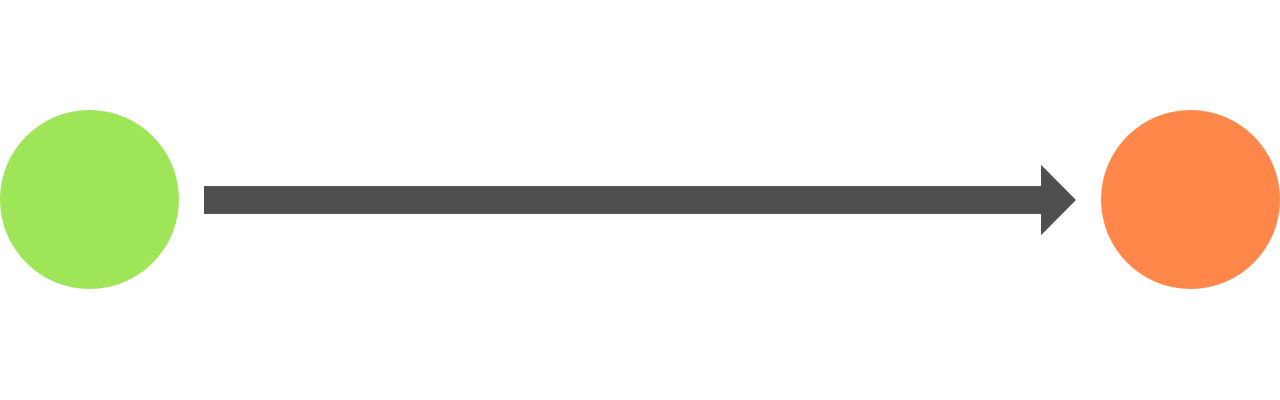
\includegraphics[width=.8\textwidth]{files/lbgArten/searchAndFind}
    \caption{Veranschaulichung des Versteckspielszenarios vgl. \cite[S. 2]{Lehmann:2012va}}
    \label{szenA}
\end{figure}

\item[Folge dem Pfad]
%\label{sec:}

Diese Variante hat Ähnlichkeiten mit einem Rennen. Ziel des Spiels ist es einer vorgegebenen Route zu folgen. Die Routen können hierbei vom Spielentwickler oder von anderen Spielern erstellt werden. Diverse Jogging-Apps arbeiten nach diesem Prinzip. Läufer A läuft beispielsweise eine bestimmte Strecke, speichert sie und andere Läufer haben dann die Möglichkeit sich mit Läufer A zu messen. Im Vorfeld muss festgelegt werden, wie Abweichungen der vordefinierten Route behandelt werden. Bei einer Jogging-App wäre es beispielsweise sinnvoll Strafpunkte in Abhängigkeit zur Größe der Abweichung von der vordefinierten Route zu verteilen. Bei anderen Apps, wäre es evtl. sinnvoller die neue Route anders auszuwerten, um so alternativ Routen anzubieten. Zusätzlich können auch alle Elemente des \textit{Versteckspiels} genutzt werden. So kann auch hier die Route auf verschiedenste Arten beschrieben werden und das Ziel kann ein bestimmtes Objektes sein. 
%\cite{creativeworklineGmbH:vb}


\begin{figure}[H]
    \centering
    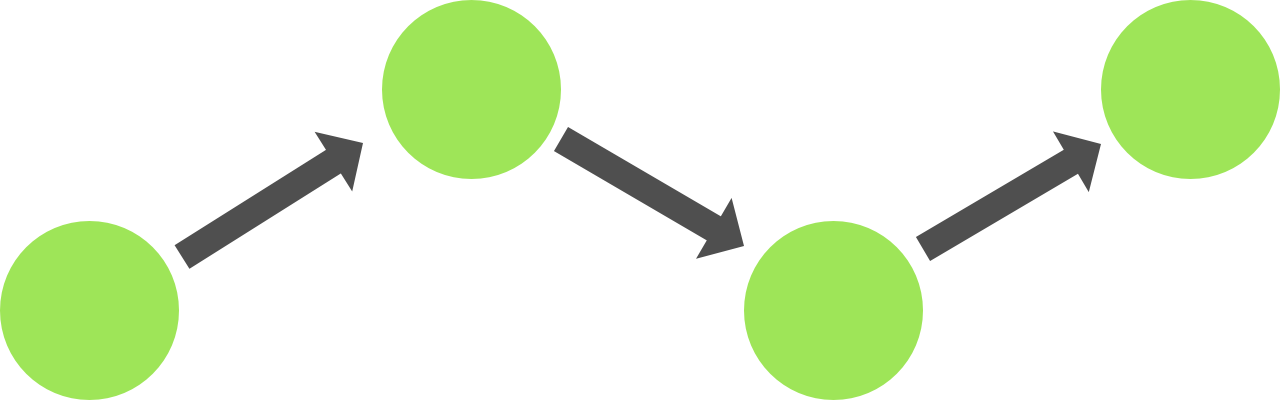
\includegraphics[width=.8\textwidth]{files/lbgArten/followThePath}
    \caption{Veranschaulichung des Folge dem Pfad Szenarios vgl. \cite[S. 2]{Lehmann:2012va}}
    \label{szenB}
\end{figure}


\item[Fangen] 
\label{sec:szenarioFangen}
Das häufig von Grund- und Vorschulkindern gespielte Spiel \glqq Fangen\grqq\ kann auch im Location-based Rahmen umgesetzt werden. Die Aufgabe des Spielers ist es ein sich bewegendes Objekt in der Spielwelt zu fangen. Dies können virtuelle Objekte sein oder andere Spieler, wodurch die Ähnlichkeit zum Kinderspiel deutlich wird. Der entscheidende Punkt hierbei ist die Bewegung des Objektes. Durch verschiedene Bewegungsmuster muss der Spieler unterschiedliche Strategien entwickeln. Bewegt sich ein Objekt z.B. im Kreis, hat der Spieler die Möglichkeit den Weg abzukürzen. Zusätzlich spielt das Intervall, in dem sich das Objekt bewegt eine weitere wichtige Rolle bei der Entwicklung der Fangstrategien.
\cite[S. 1 f.]{Misund:2009ge}

\begin{figure}[H]
    \centering
    
\includegraphics[width=.8\textwidth]{files/lbgArten/chaseAndCatch}
    \caption{Veranschaulichung des Szenarios Fangen vgl. \cite[S. 2]{Lehmann:2012va}}
    %\label{chart:alterFreizeit}
\end{figure}

\item[Bewegen]
\label{sec:szenarioPosition}
Im Gegensatz zu den drei anderen vorgestellten Szenarien ist es hier nicht von Bedeutung ein bestimmtes Ziel zu erreichen. Auch das Einhalten einer vorgegeben Route muss nicht berücksichtigt werden. Es geht darum, dass der Spieler sich bewegt. Dies lässt sich beispielsweise mit einem Spaziergang vergleichen. Auch hier kommt es nicht auf ein Ziel oder die gewählte Route an. Lediglich die Geschwindigkeit mit der sich ein Spieler bewegt, kann hierbei berücksichtigt werden. \\
Das Spiel \glqq The Journey\grqq\ der Firma \textit{Mopius} benutzt dieses Prinzip. Damit sich die Geschichte des Spiels entfaltet muss sich der Spieler fortbewegen. Der Weg ist das Ziel.
\cite{mopius:PZPdJF8n}

\begin{figure}[H]
    \centering
    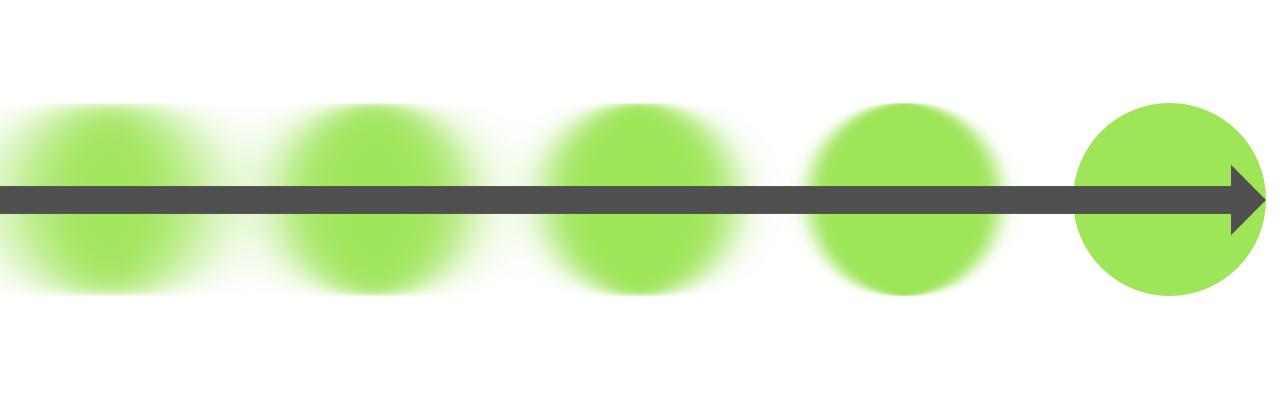
\includegraphics[width=.8\textwidth]{files/lbgArten/changeOfDistance}
    \caption{Veranschaulichung des Szenarios Positionsänderung vgl. \cite[S. 2]{Lehmann:2012va}}
    \label{szenD}
\end{figure}

\end{description}

%\section{Grayboxing / Grafik??}
%\label{sec:ext_grayboxing}
%
%Words in a novel can create images in the mind more powerful than any photograph because they only suggest an image, leaving the mind to fill in the details. A photograph demands less imagination than a novel, but also leaves less room to imagine.
%
%Showing and telling players less creates more room for apophenia to fill in the gaps.
%
%
%More detailed graphics and higher-quality sound add something to a game, but they also take something away. The more detailed the graphics, sound, and dialogue of a game, the less space there is for interpretation. The more abstract, nonspecific, and minimalistic the representation, the more apophenia becomes possible. So sometimes it’s worth deliberately communicating less so that the player can interpret more.
%
%An image in the eye overrides an image in the imagination.
%The purest example of minimalism-driven apophenia is the toy Rory’s Story Cubes. The Story Cubes are nine dice covered with cartoon pictures of sheep, lightning bolts, and other random images. Players roll the dice, look at the pictures, and make up a story that links them together. At first, it sounds absurd to try to link together pictures of a turtle, a speech bubble, and a tree. But it’s actually quite easy, especially for creative people with weak associative barriers (like children, the toy’s main target market).
%
%
%\cite[S. 93 f.]{Adams:1515529}
%
%
%Um Zeit und kosten zu sparen, kann man das so genannte Grayboxing einsetzen. Diese Technik bedeutet, dass bestimmte Teile eines Spiels, durch stark vereinfachte Modelle des finalen Modells eingesetzt werden. Oftmals werden in den ersten Testphasen eines Spiels untexturierte Level oder Levelelemente benutzt um zu schauen, in wie fern ein Level überhaupt spielbar ist. Man kann diesen Begriff aber auch ausdehnen und so zum Beispiel die Musik stark reduzieren oder ggf. ganz entfernen. Auch Charaktermodelle können durch einfache Quader oder Kugeln ersetzt werden. Somit kann schon zu Anfang der Entwicklungszeit relativ schnell Spielmechaniken getestet werden. Jedoch sollte hierbei darauf geachtet werden, dass lediglich Mechaniken getestet werden können. Spiele die stark auf Kunst, gemeint sind Visualisierung und Klangbild, ausgelegt sind, sind wesentlich schwieriger bis gar nicht "Graybox-bar", Da durch den Artstyle gezielt bestimmte Emotionen hervorgerufen werden sollen. \\ Stellt man sich das Anhand zweier Beispiele vor, wird das es deutlicher. Nimmt man ein Strategiespiel zur Hand, sind die wichtigsten Elemente der Kampf und der Aufbau. In beiden Szenarien kommt es im Grunde nur auf die implementierten Spielmechaniken an. Funktionieren alle Bounding-Box checks auch wenn sich 100 Einheiten auf dem Bildschirm befinden? Lassen sich Einheiten und Gebäude nach dem vorgegeben Schema aufrüsten? \\ Nimmt man hingegen ein Horror-Spiel, das durch seine beklemmende Stimmung dem Spieler einflößen soll, lässt sich dies nicht herausfinden. Denn der Spieler wird sich anders fühlen, wenn er in einem untexturierten Raum vor einem großen Würfel steht oder der virtuelle Pulsschlag aus den Boxen ertönt, die Musik unterbrochen wird und vor ihm ein Monster steht, das direkt aus einem seiner wildesten Alpträume entsprungen sein könnte. \cite[S. 300]{Adams:1515529}
